
%%%%%%%%%%%%%%%%%%%%%%%%%%%%%%%%%%%%%%%%%%%%%%%%%%%%%%%%
% LaTex Template for proposals within the              %
% DFG Research Unit Program                            %         
%Planet Formation Witnesses and Probes: Transition Discs
% August 2016                                            %                           
%                                                      %
%%%%%%%%%%%%%%%%%%%%%%%%%%%%%%%%%%%%%%%%%%%%%%%%%%%%%%%%
%
% 
%
% This template may be used to prepare proposals in latex.
%
%
% The project description, including publication list, should be no more than 20 pages
% in length. It should be self-explanatory and not require reviewers to read the 
% literature that is quoted or enclosed.

\documentclass[10pt,fleqn,twoside]{article}

%%%%%%%%%%%%%%%%% GET THE STYLE STUFF %%%%%%%%%%%%%%%%%%%

%%%% USE ARIAL FONT %%%%%%%%%%%%%%%%%%%%%%%%%%%%%%%%%%%%%%%%%%%%%%%%%%%%%%
\usepackage{helvet}
\renewcommand\familydefault{phv}

%%%% INCLUDE NECESSARY PACKAGES %%%%%%%%%%%%%%%%%%%%%%%%%%%%%%%%%%%%%%%%%%
%\usepackage{babel}
\usepackage[UKenglish]{babel}
\usepackage{amsmath}
\usepackage{amssymb}
\usepackage{fancyhdr}
\usepackage{natbib}
\usepackage{ae,aecompl}
\usepackage{graphicx}
\usepackage{palatino}
\usepackage[T1]{fontenc}
\usepackage[right]{eurosym}
\usepackage{rotating}
\usepackage{epsf}
\usepackage{setspace}
\usepackage{xspace}
\usepackage{multicol}
\usepackage{siunitx}
%\usepackage{caption}

\usepackage{sfmath}

\usepackage[utf8]{inputenc}

% ========= hyperref & Colors & Links ===========
\usepackage[usenames,dvipsnames]{xcolor}
%\usepackage[breaklinks]{hyperref}
\usepackage{hyperref}
\addto\extrasUKenglish{%
\def\sectionautorefname{Section}%
\def\subsectionautorefname{Section}%
\def\subsubsectionautorefname{Section}%
\def\paragraphautorefname{Section}%
}
\usepackage[all]{hypcap} % fixes links to floats
\usepackage{aas_macros}  %
\setlength{\bibsep}{-0.5pt}

% ========= highlighting important parts of the proposal ===========
\definecolor{HighLight}{rgb}{0.9,0.3,0.0}
%\newenvironment{highlight}{\color{blue}\itshape}{\ignorespacesafterend}
%\newenvironment{highlight}{\color{RedOrange}\itshape}{\ignorespacesafterend}
%\newenvironment{highlight}{\color{RedOrange}\bfseries}{\ignorespacesafterend}
%\newenvironment{highlight}{\color{BrickRed}\bfseries\itshape}{\ignorespacesafterend}
%\newenvironment{highlight}{\color{BrickRed}\bfseries}{\ignorespacesafterend}
%\newenvironment{highlight}{\color{HighLight}\bfseries}{\ignorespacesafterend}
\newenvironment{highlight}{\color{HighLight}}{\ignorespacesafterend}
\newenvironment{missingenv}{\color{red}}{\ignorespacesafterend}

\definecolor{Emphasize}{rgb}{0.0,0.5,0.0}
\newenvironment{Emphasize}{\color{Emphasize}\itshape}{\ignorespacesafterend}


% strike through comments: to turn them off, uncomment the renewcommands below
\usepackage{soul}
\setstcolor{red}

% ========= Commands specially for the forschergruppe =========

\newcommand{\todo}[1]{\textcolor{red}{\bf #1}}
\newcommand\connect[1]{{\color{OliveGreen} #1}}

%%%% CAPTION LAYOUT %%%%%%%%%%%%%%%%%%%%%%%%%%%%%%%%%%%%%%%%%%%%%%%%%%%%%

\usepackage[font={small}]{caption}

%%%% PAGE LAYOUT %%%%%%%%%%%%%%%%%%%%%%%%%%%%%%%%%%%%%%%%%%%%%%%%%%%%%%%%%
\setlength{\textheight}{22cm}
\setlength{\topmargin}{-1.2cm}
\setlength{\textwidth}{15.6cm}
\setlength{\oddsidemargin}{0.0cm}
\setlength{\evensidemargin}{0.0cm}
\setlength{\mathindent}{1.5cm}
\setlength{\parindent}{0.0cm}
\setlength{\parskip}{0.08cm}

%%%% PAGE HEADER %%%%%%%%%%%%%%%%%%%%%%%%%%%%%%%%%%%%%%%%%%%%%%%%%%%%%%%%%%
\pagestyle{fancy}
\fancyhead[RE,RO]{}
\fancyfoot[RO]{\thepage}
\fancyfoot[LE]{\thepage}
\fancyfoot[CE,CO]{}

%%% FONTS FOR THE TITLE PAGE %%%%%%%%%%%%%%%%%%%%%%%%%%%%%%%%%%%%%%%%%%%%%%
\newfont{\tpfonta}{cmssbx10 scaled 1600}
\newfont{\tpfontb}{cmssbx10 scaled 3200}

%%%% COLOR DEFINITIONS %%%%%%%%%%%%%%%%%%%%%%%%%%%%%%%%%%%%
\definecolor{blue} {rgb} {0.25,0.25,0.75}

%%%% ADDITONAL EMPHASIS %%%%%%%%%%%%%%%%%%%%%%%%%%%%%%%%%%%
\newcommand{\cem}{\color{blue}}
\newcommand{\eem}{\sl\color{blue}}

%%%% BIBTEX PUNCTUATION %%%%%%%%%%%%%%%%%%%
\bibpunct{(}{)}{;}{a}{}{,} % to follow the A&A style

%%%% SET THE COLOR OF THE (SUB-) SECTION TITLES %%%%%%%%%%% 
\newcommand{\Tcol}{\color{blue}}

%%%% SET THE COLOR OF THE TITLE BOX BACKGROUND %%%%%%%%%%%%
\definecolor{Background}{rgb} {0.62,0.75,0.5}

%%%%%%%%%%%%%% REFERENCE SECTION NAME %%%%%%%%%%%%%%%%%%%%
\renewcommand\refname{\Tcol 9. Bibliography}

%%%%%%%%%%%%%% NICER PROJECT REFERENCES %%%%%%%%%%%%%%%%%%%

\newenvironment{literature}%
 {\begin{multicols}{2}\begin{scriptsize}\begin{list}{}{%
   \setlength{\topsep}{0em}%
   \setlength{\parskip}{0em}%
   \setlength{\parsep}{0em}%
   \setlength{\itemsep}{0em}%
   \setlength{\rightmargin}{0em}%
   \setlength{\leftmargin}{2em}%
   \setlength{\itemindent}{-2em}}}%
 {\end{list}\end{scriptsize}\end{multicols}}

%
% ...A compact itemize environment
%
\newenvironment{compactitemize}%
 {\begin{list}{$\bullet$}{%
   \setlength{\topsep}{0em}%
   \setlength{\parskip}{0em}%
   \setlength{\parsep}{0em}%
   \setlength{\itemsep}{0.0\baselineskip}%
   \setlength{\rightmargin}{0em}%
   \setlength{\leftmargin}{2.0em}%
   \setlength{\labelsep}{0.5em}%
   \setlength{\labelwidth}{1em}%
}}
 {\end{list}}

\newcounter{qcounter}
\newenvironment{compactenumerate}%
 {\begin{list}{\arabic{qcounter})~}{\usecounter{qcounter}%
   \setlength{\topsep}{0em}%
   \setlength{\parskip}{0em}%
   \setlength{\parsep}{0em}%
   \setlength{\itemsep}{0.0\baselineskip}%
   \setlength{\rightmargin}{0em}%
   \setlength{\leftmargin}{2.0em}%
   \setlength{\labelsep}{0.5em}%
   \setlength{\labelwidth}{1em}%
}}
 {\end{list}}

%%%% EXPLANATION FOR THE CONNECT COLOR %%%%%%%%%%% 
\newcommand{\footexplainconnect}{\footnote{The text highlighted in \connect{green} refers to the connection of this project to other projects of this Research Unit.}}
 
%%%%%%%%%%%%%%%%%% NICER REFERENCES %%%%%%%%%%%%%%%%%%%

%\usepackage[capitalise,nameinlink]{cleveref}
\newcommand{\cref}[1]{\autoref{#1}}

%%%%%%%%%%%%%%%%%% COLOR THE SECTION NUMBERS %%%%%%%%%%%%%%%%%

\makeatletter
\renewcommand\@seccntformat[1]{\color{blue} {\csname the#1\endcsname}\hspace{0.5em}}
\makeatother
\renewcommand\thesection{\arabic{section}.}
\renewcommand\thesubsection{\arabic{section}.\arabic{subsection}}

%%%%% color sections
\usepackage{sectsty}
\allsectionsfont{\color{blue}}


%%%% CHANGE THE APPEARANCE OF THE \PARAGRAPH COMMAND  %%%%%%%%%%%%%%%%%%%%%%%%%%%%%%%
\makeatletter
\renewcommand\paragraph{\@startsection{paragraph}{4}{\z@}%
            {-2.5ex\@plus -1ex \@minus -.25ex}%
            {1.25ex \@plus .25ex}%
            {\normalfont\normalsize\bfseries\Tcol}}
\makeatother
\setcounter{secnumdepth}{4}     % how many sectioning levels to assign numbers to
\setcounter{tocdepth}{4}        % how many sectioning levels to show in ToC

%%%%% set header

\renewcommand{\sectionmark}[1]{\markright{\color{black}#1}}

\newcommand{\caphighlight}[1]{{\bf #1}}



%%%%%%%%%%%%%%%%% DEFINE THE HEADER TEXT %%%%%%%%%%%%%%%%

\fancyhead[LE,LO]{\slshape
%%%%  Please edit
%
Leonardo Testi: Solids and gas in disks
%
%
%%%%%
}

\begin{document}


\newpage

%%%% PROJECT DESCRIPTION STARTS HERE %%%%%%%%%%%%%%%%%%%%%%%%%%%%%%%%%%%

\setcounter{page}{1}

\centerline{\huge\bf\Tcol
%
%
%
%
%%%%  Please edit
%
 Project A1: }
\vspace{1em}

\centerline{\LARGE\bf\Tcol Solids and gas evolution in disks:}\vspace{0.3em}
\centerline{\LARGE\bf\Tcol observational constraints}

%
%%%%
%
%
%
%
\vskip1.0cm

%%%%  Please edit

\noindent{\bf Authors:}\\
\begin{tabular}{ll}
{\textsf{PI:}}                   & L.~Testi (ESO)\\
%{\textsf{Co-I:}}                & B.~Ercolano (LMU), T.~Preibisch (LMU), T.~Henning (MPIA), E. van Dishoeck (Leiden, MPE)\\
%{\textsf{Collaborations:}}      & H.~Baobab~Liu (ESO),  J.M.~Carpenter (ALMA), G.~Guidi (INAF/UniFi)\\
%                                & A. Miotello (Leiden),  I.~Pascucci (Arizona), A.~Natta (DIAS/INAF),\\
%                                &  M.~Tazzari (IoA), J.P.~Williams (Hawaii), Hsi-Wei Yen (ESO)\\
{\textsf{Co-I:}}                & B.~Ercolano (LMU), T.~Preibisch (LMU)\\
{\textsf{Collaborations:}}      & H.~Baobab~Liu (ESO),  J.M.~Carpenter (ALMA), T.~Henning (MPIA),\\
                                & A. Miotello (Leiden),  I.~Pascucci (Arizona), M.~Tazzari (IoA),\\
                                & E. van Dishoeck (Leiden, MPE), J.P.~Williams (Hawaii)\\
\end{tabular}

\vspace{1em}
\noindent{\bf Requested positions: 2 PhD students} \\

\vspace{1em}
\noindent{\bf Abstract:}\\
This project aims at obtaining observational constraints on the dust and gas 
properties of protoplanetary discs as a function of evolutionary stage (e.g.\ primordial to transition) and 
the physical properties of the central star. We will analyse systematically
the ALMA observations of young stars with discs in nearby star forming regions already collected as part of a series of programmes and we will complement these with additional 
ALMA and VLA observations. We will firmly characterize the level of grain growth and the gas content as traced by CO and isotopologues in discs as a function of stellar mass, evolutionary stage and morphology of the disc, and we will search for evidence of disc-planet interaction in the discs structure and kinematics of transitions discs. We will provide direct observational tests of different planetesimal formation theories and how/if they apply in different environments.

\section{State of the art and preliminary work}
\renewcommand{\leftmark}{\sc State of the Art and preliminary work}
\label{s_state_art}

The aim of this project is to provide an observational characterization of the dust and molecular gas
(as traced by CO and its isotopologues) in transition disks as part of the global population of protoplanetary disks in nearby star forming regions.  

Transition Disks (TDs) are generally observationally defined based on the observed Spectral Energy
Distribution (SED) and disk sub-mm morphology which are characteristic of disks with an inner region
with low dust opacity. There is still uncertainty on their relation 
to disk evolution and planet formation, but are generally thought to be a transition phase that
primordial full disks undergo as they are dissipated (see e.g.\ Williams \&\ Cieza 2011). In recent 
years the brightest disks with the largest holes have started to be characterized with high angular resolution submm continuum and spectral line observations. 
Pre-ALMA observations have been used to quantify the dust surface density drop required to 
explain the observed inner cavities (e.g.\ Andrews et al.~2011), and ALMA is now allowing a more 
detailed study of the molecular gas content (e.g.\ van der Marel et al.~2015). 
The relationship between TDs and dust evolution and planet formation has also started to be investigated,
but with very limited studies so far (e.g.\ Pinilla et al.~2014, Sallum et al.~2015).
These initial studies have provided fundamental insights on the properties of TDs, but a 
systematic comparative study with the properties of the global population of disks in different 
star forming regions is lacking. With this project we propose to make full use of the ALMA and VLA capabilities complemented by high contrast infrared observations at the LBT and VLT. These facilities 
are now providing us the possibility to perform comparative demographical studies of full samples of young evolving populations as well as detailed analysis planet forming disks in different evolutionary stages. 

A systematic assessment of the properties and evolution of dust and gas in TDs as compared with the rest of the disk population is required to constrain the nature of TDs and their relation to the global disk evolution and planet formation process. Four main properties need to be studied and can now be constrained 
observationally: the dust properties and distribution, the gas properties and distribution, the wind and accretion properties, and the presence and properties of planets. These properties are related to the evolution of disks and the formation of planets: dust grains are expected to grow to pebbles and planetesimals and eventually form the cores of planets; the disk gas content is the reservoire out of which planetary atmospheres are formed, its evolution is linked to the interplay between planet formation and disk dispersal; accretion onto the central star and the wind properties are key observables to compare with disk dissipation models; the effects of planets on the disk, once they are formed, can profoundly influence the future ability of the disk to form planets and its dissipation.

Detailed studies of few TDs exist on all the aspects above (see Fig.~\ref{f_examples} for the case of LkCa15, one of the very few TDs with directly imaged planets inside the inner cavity), but it is now possible to explore the properties of TDs in the broader context of the demographics of planet forming disks as a function of age and as a function of the properties of the central star.  
\begin{figure}
\centerline{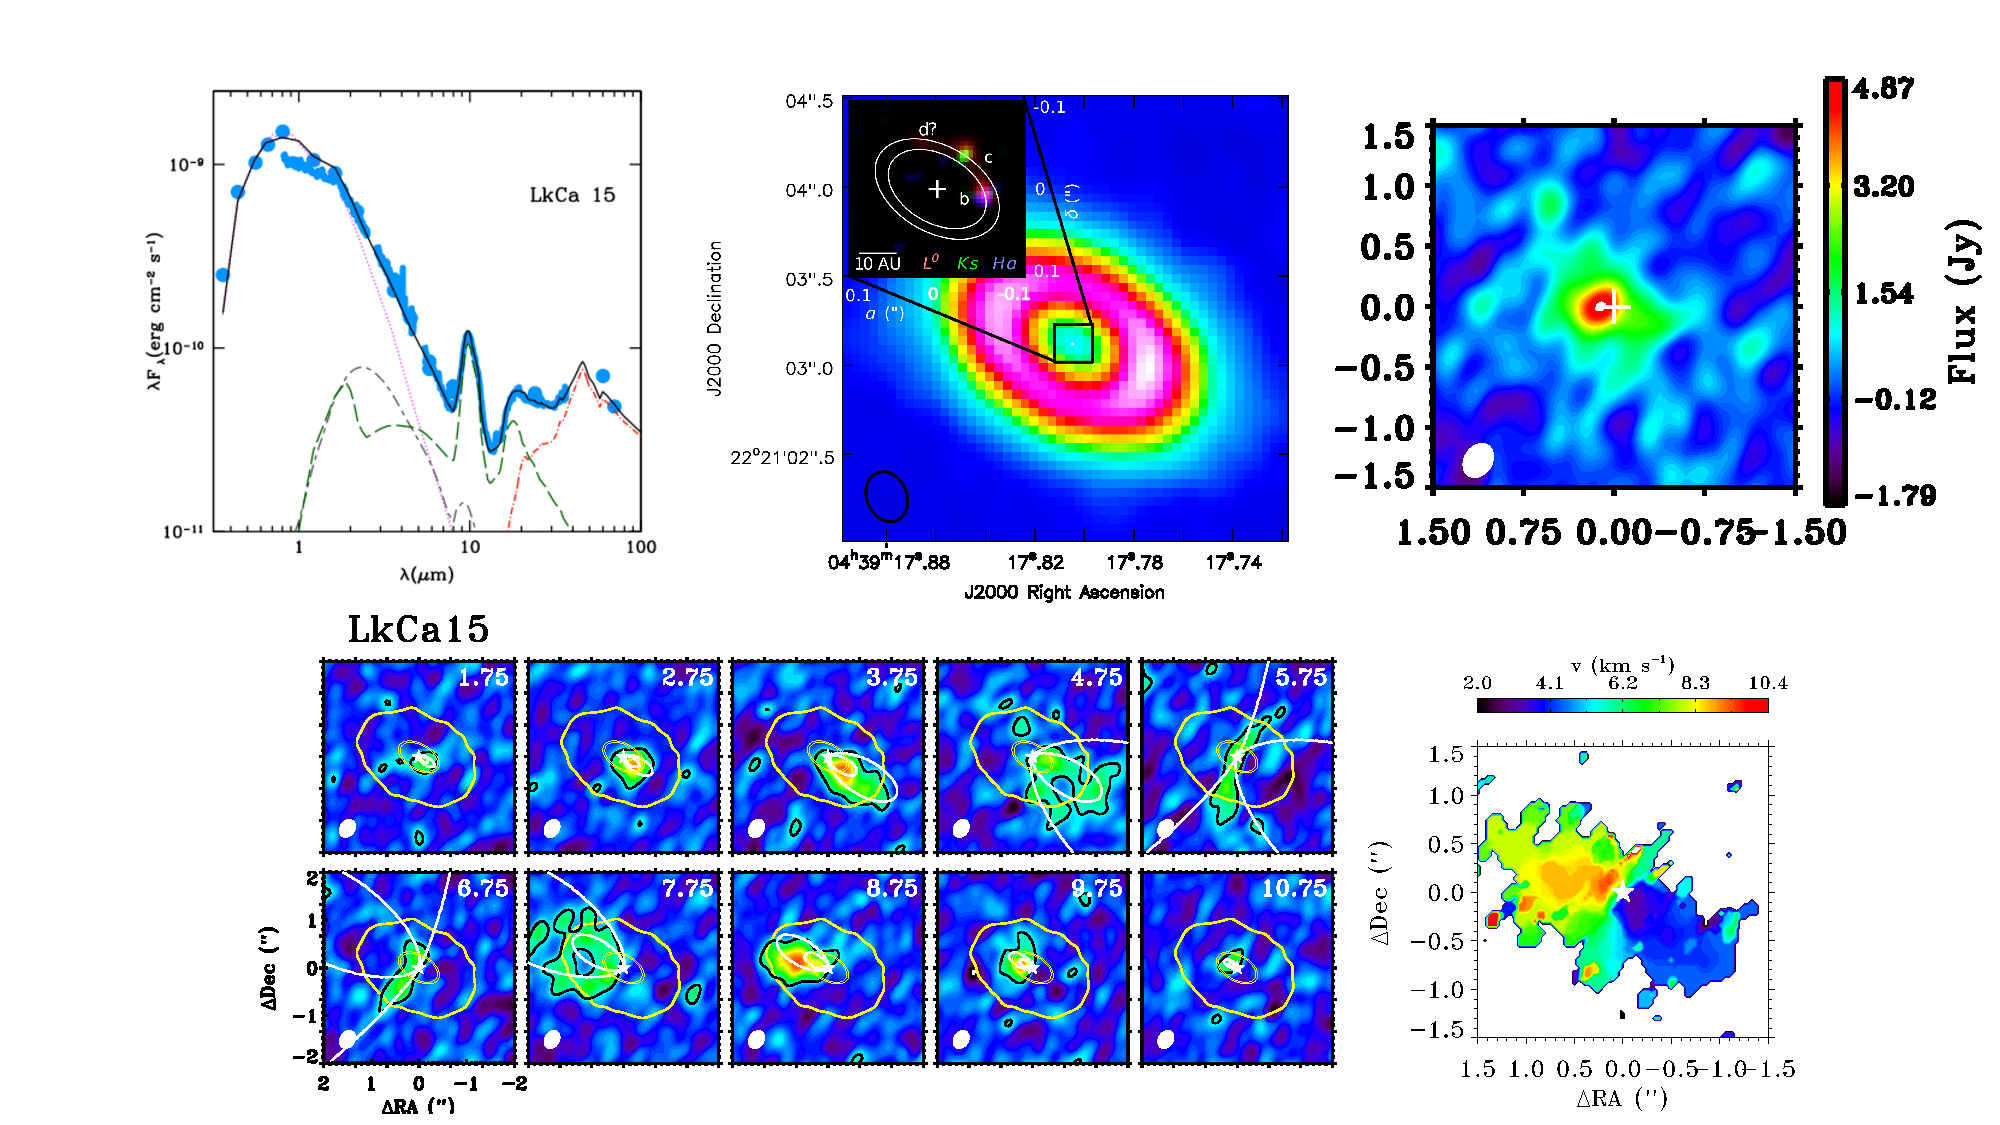
\includegraphics[scale=0.5]{Figure_LkCa15.pdf}}
\caption{The LkCa15 Transition Disk. \caphighlight{From left to right and
    top to bottom:} SED of the LkCa15 system showing the characteristic dip
  of Transition Disks in the mid-infrared , followed by a rise at
  far-infrared wavelengths (Espaillat et al.~2011); ALMA dust continuum
  image, showing the characteristic inner hole (in this case the cavity
  outer radius is $\sim$45~AU), the inset shows the location of the young
  planets detected in this system (Sallum et al.~2015); the ALMA
  observations of $^{12}$CO(6-5) observations show the presence of warm gas
  inside the cavity (van der Marel et al.~2015).}
\label{f_examples}
\end{figure}

In the following four subsections, we summarize the state-of-the-art of our observational constraints on the four main properties outlined above and point out one key question in each area that we will address as part of this project and in collaboration with the rest of the RU teams.

\subsection{Dust properties and distribution} 
The properties of the dust distribution is the main observable quantity that sets the TDs class apart form the rest of the disk population. The presence of a hole in the dust distribution can be inferred from the SED, and the hole size roughly constrained through modeling, but only direct imaging at (sub-)millimetre imaging.
Grain growth is a stage of planet formation that can be directly observed due to the effects on particle emissivity. Planetesimals and early planetary cores formation are difficult to probe observationally, while growing planetary bodies can be studied through their influence on the disc structure or directly imaged in the outer disc, when sufficiently young and large.

Submillimetre and centimetre wave observations over the last decade have established that grain growth occurs very early in the protoplanetary discs lifetime, large grains and pebbles are present in discs throughout their lifetime. This is at odds with simple grain evolution theories in gaseous discs, and several ideas have been put forward to explain this fact. Modern theoretical models require large grains confinement in specific regions of the disc associated with local pressure maxima in the gas phase transitions of abundant molecules (snowlines), or regions with very low gas to dust ratio. The new ALMA high angular resolution observations of the protoplanetary discs suggest that small rocky proto-planets may form early and help trapping millimetre and centimetre-size grains in discs (HL~Tau, ALMA Partnership 2015), in other cases there is compelling evidence for more massive planets affecting the disk dust and gas distribution (Perez et al.~2016; Isella et al.~2016).  

As of today, relatively few and bright (massive) disks have direct measurements of the inner hole from sub-mm imaging
and even fewer constraints on the dust properties in the disk. The most comprehensive catalog of candidate TDs, based on SED modeling, is that of van der Marel et al.~(2016), which includes over 130 high probability TDs in nearby star forming regions. However, for the small fraction of disks with inner cavity measurements from mm interferometry the correlation between the inferred hole sizes from the SED and the sizes from direct imaging show a large dispersion (see Figure~\ref{f_TDsiz}). 
\begin{figure}
\centerline{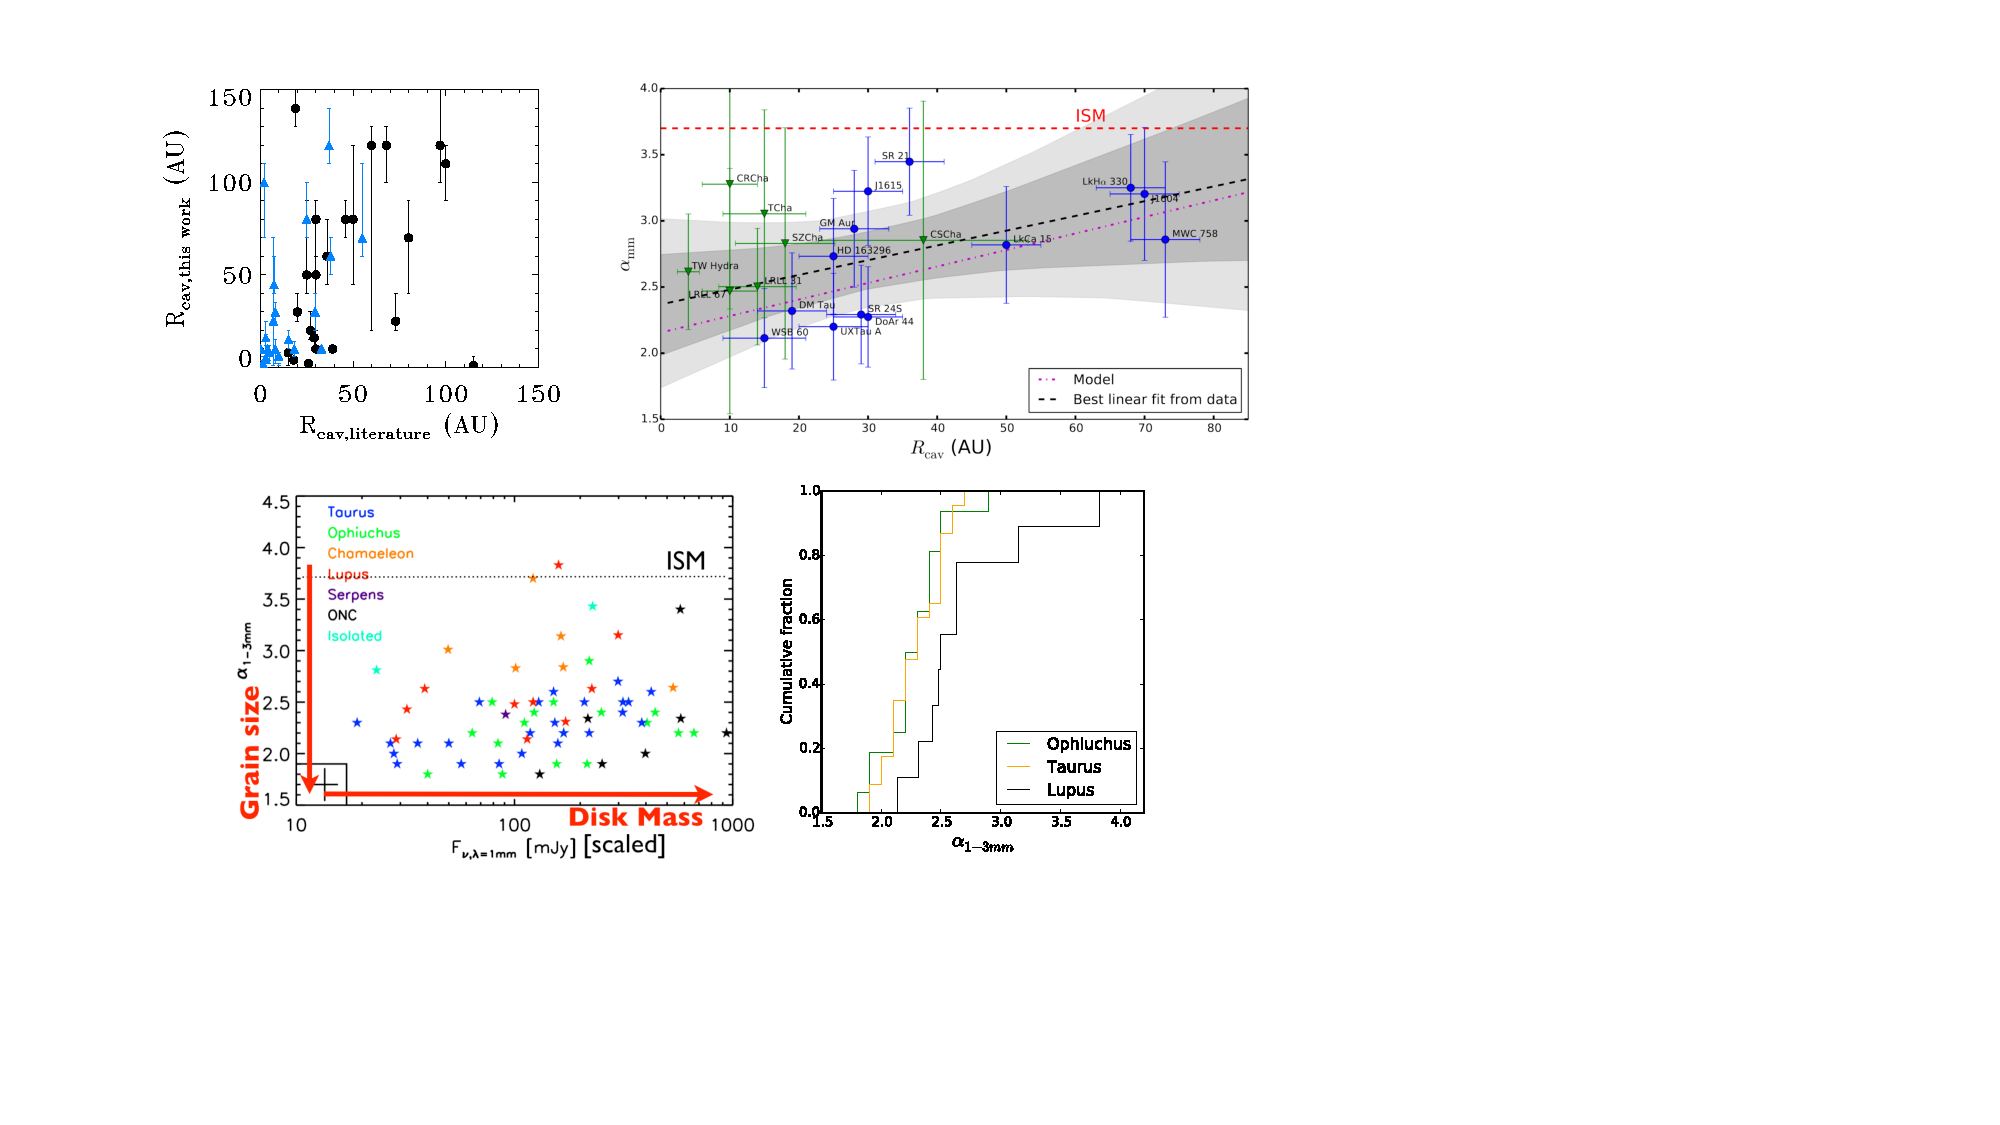
\includegraphics[scale=0.7]{f_dust_radii_tds.pdf}}
\caption{\caphighlight{Top left:} TDs hole sizes as derived from SED fitting
  and direct imaging (black points only; adapted from van der Marel et
  al.~2016a). \caphighlight{Top right:} relationship between TDs hole radius
  and mm spectral index (as a proxy of grain growth in disks, large grains
  correspond to small values of $\alpha$; adapted from Pinilla et
  al.~2014). \caphighlight{Bottom left:} compilation of pre-ALMA photometric
  estimates of grain growth in disks from millimetre spectral indices
  (adapted from Testi et al.~2014). \caphighlight{Bottom right:}
  distributions of the mm spectral indices for objects in the young
  Taurus/Ophiuchus regions (yellow/green lines, data from Ricci et
  al.~2010ab), and the slightly more evolved Lupus region (black line, data
  from Lommen et al.~2007 and Ubach et al.~2012).}
\label{f_TDsiz}
\end{figure}
Using the scant and limited quality data available so far, Pinilla et al.~(2014) showed a potential correlation between the average dust properties in TDs and the size of the inner cavity. This result is consistent with a scenario in which inside-out planet formation consumes the large grains in the inner regions of the disk to form planets, and, as the disk is progressively evacuated by planets and photoevaporation, the average dust properties are dominated by smaller grains in the outer regions of the
system. Nevertheless, there are still large uncertainties and biases on the measurements of TDs hole sizes and on the dust properties. In addition, there is marginal evidence for the dust properties to vary in different star forming regions (see Figure~\ref{f_TDsiz}, bottom panels), hence to properly understand TDs  evolution it is necessary to compare with the dust properties of the full disk populations in the same star forming regions.

\smallskip
{\bf Q1:} {\it Can we trace the evolution of the grain size distribution in full disks and TDs as disk dissipation and planet formation progress?}

\subsection{Gas properties}
Most of the primordial disk mass is in the form of molecular gas. As cold H$_2$ is not directly observable due to the lack of a permanent dipole moment, the gaseous component of the disks can only be traced by the much less abundant molecules. CO is the prime tracer of molecular gas in planet forming disks. The few TDs with detailed gas observations from ALMA show that in many cases the inner cavities are not empty, but contain warm gas, while the outer disk is rich in cold molecular gas, as primordial disks (van der Marel et al.~2015). Nevertheless, our current understanding is not yet clear-cut: quantifying the amount of gas inside the inner hole and in the outer disk are essential to provide constraints on the ability of disks to form and interact with planets and for the disk dissipation models.

The characterization of the gas contents of disks during their evolution is an area that is being profoundly transformed by ALMA: for the first time we have the sensitivity to study large samples.
Our group made a key contribution in this area in 2016 with the results of the Lupus ALMA Disks Survey
(Ansdell et at.~2016): for the first time an almost complete and unbiased sample of planet forming disks in continuum and gas was used to estimate the demographics of disk gas properties in an entire star forming region for TDs and full disks. The picture that we derive from an accurate analysis combining dust and $^{13}$CO/C$^{18}$O(3-2) emission and detailed modelling of the gas (including selective photodissociation and freezing out) is intriguing in many respects: the gas-to-dust ratios that we derive from modeling the CO are lower by one or two orders of magnitudes as compared to expectations; there is no significant difference in this result between TDs and normal disks (see Fig.~\ref{f_LADS}; Ansdell et al.~2016; Miotello et al.~2016). There are cases in which full disks show an apparent hole in the CO isotopologues (e.g.\ see the example in Fig.~\ref{f_LADS}), most likely this is the effect of continuum optical depth suppressing the line emission (see also Isella et al.~2016), which emphasizes the importance of a detailed modeling of the disk emission to extract the gas properties.

\begin{figure}
\centerline{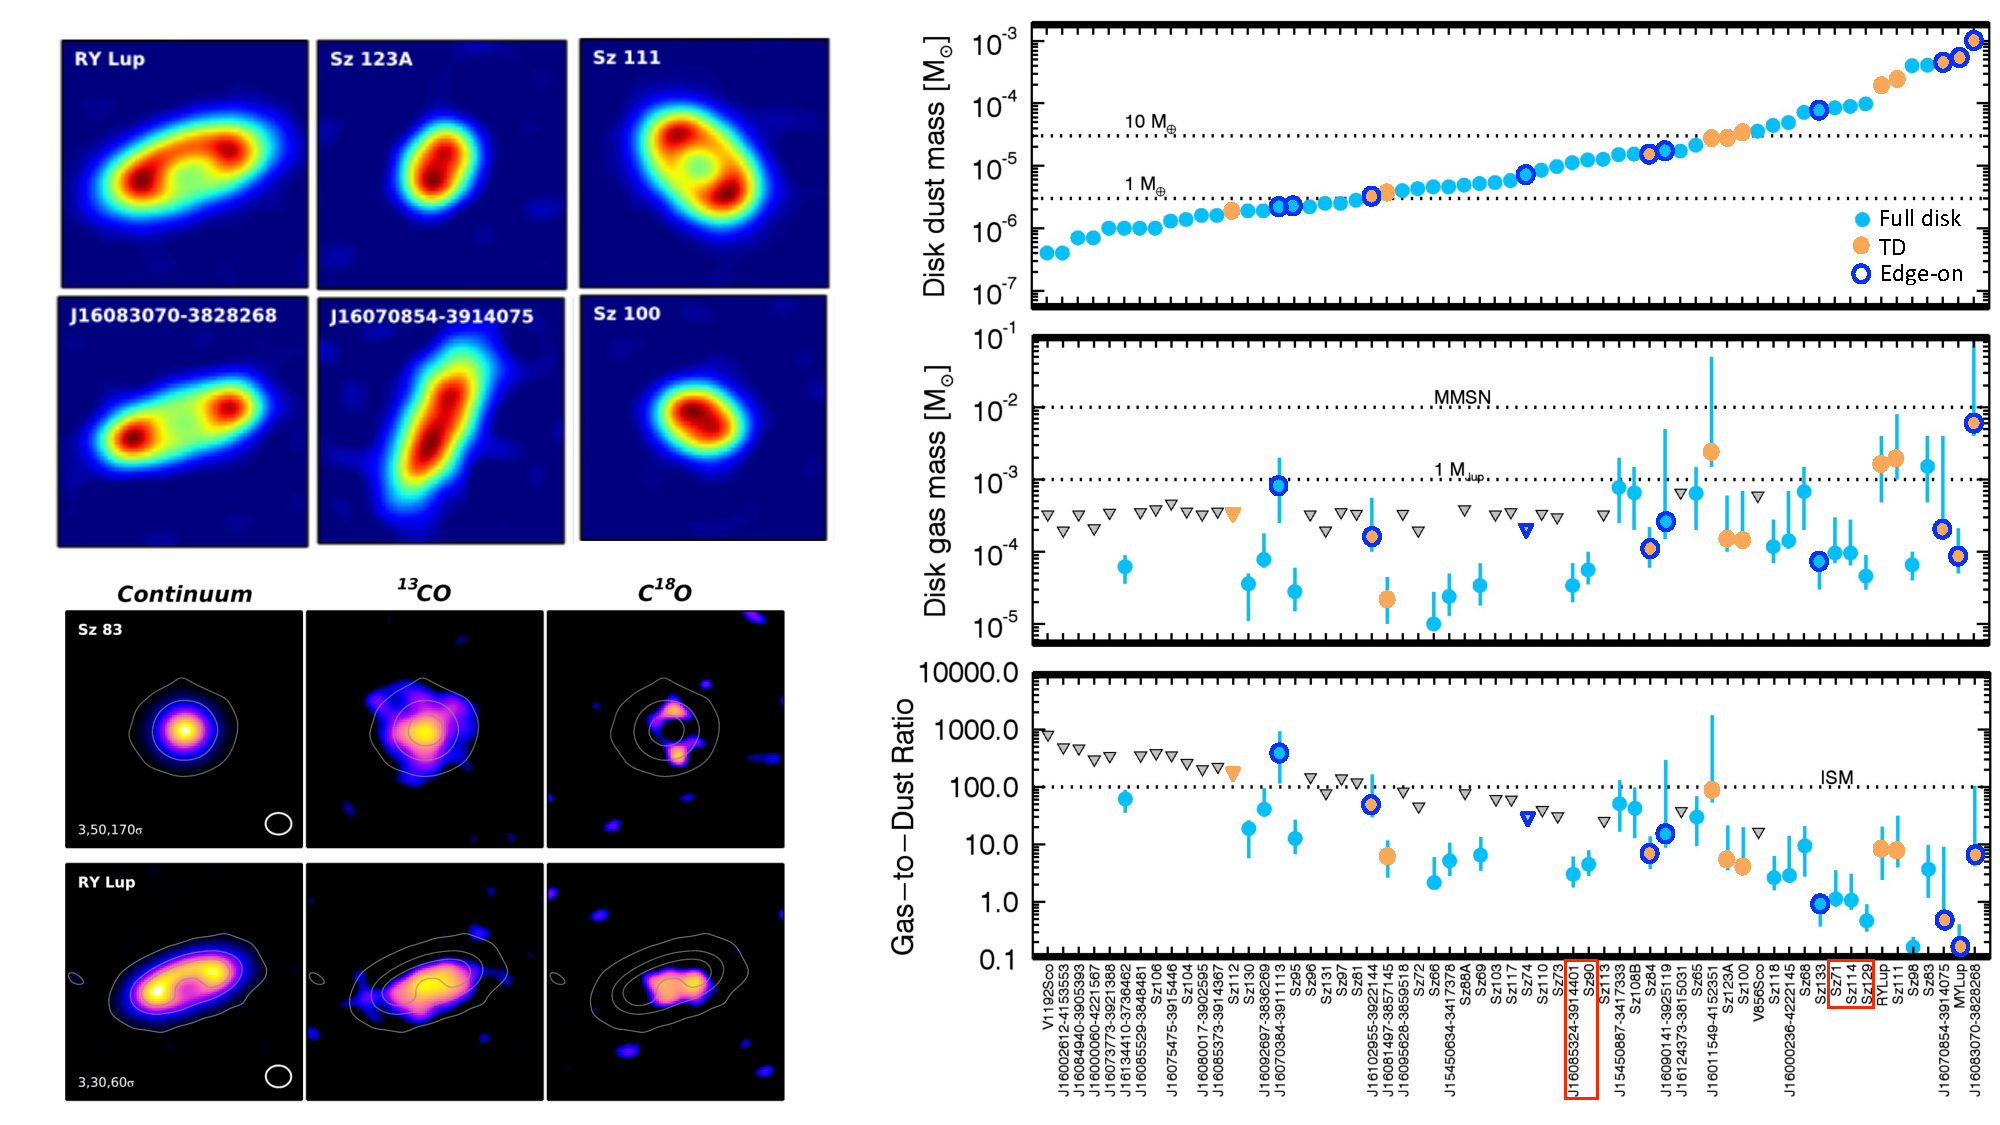
\includegraphics[scale=0.45]{Figure_Lupus_TDs.pdf}}
\caption{\caphighlight{Top left 6 panels:} ALMA 890~$\mu$m continuum images
  of six of the TDs in Lupus (LADS survey; adapted from Ansdell et
  al.~2016). \caphighlight{Bottom left panels:} Comparison of the LADS
  continuum (left colormap and contours in all panels) and $^{13}$CO (center
  colormaps) and C$^{18}$O (right colormaps) for a full disk (top) and a TD
  (bottom), note that the C$^{18}$O emission fills the inner hole in the TD
  (adapted from Ansdell et al.~2016). \caphighlight{Right panels:} From top
  to bottom: dust disk mass, gas disk mass (as derived from CO modeling),
  gas to dust ratio; TDs are shown as orange circles, while full disks are
  blue symbols, grey triangles are upper limits (adapted from Miotello et
  al.~2016).}
\label{f_LADS}
\end{figure}

The LADS results are tanatalizing, but they need to be followed up to understand the caused of the low gas-to-dust ratio as measured from the CO isotopologues.

Two other surveys of disks in nearby star forming regions have been completed (Upper Sco, Barenfeld et al.~2016, and Chamaeleon~I, Pascucci et al.~2016), but have not yet been fully analysed for the molecular gas content. ALMA data for two additional surveys of RCrA and $\sigma$Ori have been obtained by our group, the data is expected to be delivered to us in Winter 2016-2017. A complete survey of the Ophiuchus disk population is being carried out by another group, we expect the data to become publicly available in mid-2018.

\smallskip
{\bf Q2:} {\it can we trace the evolution of molecular gas as a function of disk evolution and in TDs as disks are dissipated and planet formation is occurring?}

\subsection{The disk-wind-accretion connection}

Three mechanisms are considered to be the possible main drivers of disk evolution: viscosity,
magnetically driven disk winds, and photoevaporation. Each one modifies the disk structure with 
time in a different fashion. Viscous theory (e.g.\ Lynden-Bell \&\ Pringle 1974) describes how
turbulence redistributes the disk material and the angular momentum. This results in an inward 
flow of disk material, which eventually accretes onto the star. The initial intense accretion 
rate ($M_{acc}>10^{-6}$~M$_\odot$/yr)
slows down on timescales of $\sim 1$~Myr to $M_{acc}\le 10^{-8}$~M$_\odot$/yr,
and the circumstellar disk then slowly evolves until it 
becomes optically thin on timescales $\sim$10~Myr (e.g.\ Hartmann et al. 1998). Viscous 
evolution is able to explain the general evolution of disks, and we have recently observationally confirmed a basic prediction of this theory, the existence of a correlation between $M_{acc}$ 
and the disk mass (Manara et al. 2016; see also the theoretical predictions of 
Dullemond, Natta \&\ Testi 2006), as measured through the {\it dust} emission. This 
finding supports the idea that viscous evolution may be the main ingredient of early disk evolution.
Nevertheless, there are still some major caveats that need to be understood:
the correlation between  M$_{dust}$ vs. $M_{acc}$ is {\it not} the expected one, as it is the gas,
not the dust, that is supposed to be viscously evolving, in addition
the timescale for the disk dispersal predicted from this theory is not in agreement with 
observations, and the origin of the turbulence in disks is still unclear 
(e.g.\ Turner et al. 2014). In addition, resolved disk observations with ALMA or 
near-infrared high-resolution imaging (e.g., SPHERE) show structures, such as holes and 
spirals, as well as inhomogeneities in the gas and dust distribution that cannot be 
explained by viscous evolution alone (e.g.\ Benisty et al. 2015). 

Observations of disks show that they eject large amounts of material in the form of wide-angle, 
slow winds, collimated jets, and molecular outflows (e.g.\ Frank et al., 2014; 
Bacciotti et al. 2011). These ejections are driven by the magnetic field in the disk, which gives 
rise to magnetically driven winds and jets, remove angular momentum from the disk and thus 
drive accretion in the disk and onto the central star (Ferreira et al 2006; Pudritz et al. 2007). 
These disk winds have been recognized recently as fundamental ingredients for the disk 
evolution (Armitage et al. 2013; Bai 2016). Indeed, they can accomodate the main features 
of disk 
accretion and the timescales of disk dispersal. Moreover, theoretical work is showing that 
disk winds have a strong impact on planet formation, since they can inhibit the drift of 
grains and type-I migration of planets (Suzuki et al., arXiv:1609.00437). However, 
quantitative constraints on this theory are still lacking because MHD simulations are 
local and not global, and the large number of free parameters makes these predictions 
still qualitative. In addition, photoevaporative winds accelerated from the disk surface 
by high energy X-ray and UV photons coming from the central star are dominant at late 
stages when accretion has decreased. Migration of planets may be stopped at $\sim$1-2~au 
from the central star in disks affected by photoevaporation, thus explaining the observed 
peak in the exoplanet semi- major axis distributions (Alexander \&\ Pascucci 2012; 
Ercolano \&\ Rosotti 2015). Photoevaporation explains the rapid final disk dispersal 
and formation of holes in TDs (e.g.\ Alexander et al. 2014), but falls short in explaining 
accretion in objects with large cavities (Owen \&\ Clarke 2012).

On the observational side, our work (Manara et al. 2016) has shown that stellar photospheric parameters and mass accretion rates can now be derived from optical/infrared spectroscopy with sufficient 
accuracy to start testing the predictive theories. As part of our ongoing efforts, our group has 
been acquiring optical/infrared spectroscopy of large samples of objects for large samples of 
star-disk systems in nearby star forming regions. These data will be available to complement the 
ALMA data on the gas and dust properties of full disks and TDs. We will be able to address the 
potential correlation between disk properties and mass accretion rate and to search for an 
evolution or deviation from the naive expectation of viscous evolution theories connected to the 
effects of disk winds and photoevaporation, and the formation of TDs.

\smallskip
{\bf Q3:} {\it can we trace the transition from viscous dominated to disk wind and photoevaporation dominated evolutionary phase in disk and TDs?}

\subsection{Presence and properties of planets}

Observational studies and simulations of TDs suggest that the presence of planetary-mass companions within the inner hole may be common, and indeed, in a few cases of TDs there are clear observational indications (e.g.\ Reggiani et al. 2014; Sallum et al. 2015, see also \ref{f_examples}; van der Marel 2016b).
Nevertheless, 
as outlined above, ALMA is now revolutionizing our view of FULL disks as it allows for the first time to resolve in exquisite detail the solids and distribution and reveal the process of planet formation as it unfolds.

High angular resolution continuum observations of protoplanetary full disks with ALMA reveal a variety of small scale structures. The most famous and dramatic example is the ring system around the young star HL~Tau (ALMA Partnership 2015), but many more are being published by various groups from the PI-science observations of dust distributions in disks at 1.3mm and/or 890$\mu$m at 0.05-0.1~arcsec angular scales (e.g.\ TW~Hya, Andrews et al. 2016; HD163296, Isella et al. 2016; Elias~2--27, Perez et al. 2016; among many others). The variety of single wavelength millimetre continuum morphologies observed so far is very broad: dark rings, with variable depth and location, and spiral structures with different contrasts and threads, with and without inner rings. Particularly relevant in this context are the observations of Isella et al.~(2016), who showed that the gaps observed in the dust distribution are also associated with depressions in the gas surface density, indicating the presence of relatively large planets.

A key feature, first suggested by the observations of HL Tau, seems to be that planet formation in the outer disk (R$\ge$10-20~AU) can occur very early in the disk life, much earlier than the typical 2-3~Myr lifetime. This could be the result of planet formation via gravitational instabilities in massive young disks. Massive planets (M$\ge 1-5$~M$_{Jup}$) formed by gravitational instabilities in the outer disk should be able to quickly open gaps in the disk leading to some of the observed features. More specifically, recent simulations on embedded planets in dusty disks, suggest that the minimum planetary mass needed to carve a gap in both dust and gas is as low as 1 to a few M$_{Jup}$, depending on the parameters of the system (Dipierro et al. 2016, see Fig.~1). Young planets down to $\sim$1~M$_{Jup}$ should then be observable through the gaps they open in the disk using state-of-the-art thermal and near infrared high contrast imaging instruments at large telescopes. We have initiated a survey program using LBT/LBTI and VLT/SPHERE to survey for planetary mass companions in planet forming disks that show dust and gas gaps and holes with ALMA high angular resolution observations. The initial results demonstrate the possibility to achieve the goal of detecting Jupiter-mass companions in the outer disk.

\smallskip
{\bf Q4:} {\it are $\ge$1~M$_{Jup}$ planets common in planet forming disks and which is their relationship with the observed distribution of dust and gas in full disks and TDs?}

\subsection{Project-related publications}

% Please list your own publications related to the proposed project, 
% adhering to the rules of the DFG guidelines 1.91. In brief, please note: 
% - Up to 10 publications
% - The work must be published or accepted.
% - Publications on astro-ph (arXive, SPIRES or articles with a DOI) count as published. 
% - Any work that is only in the status ``accepted'' MUST be attached to the proposal
%    together with the acceptance letter.
% - All publications in this section CAN be attached to the proposal. Please limit these
%    attachments to a minimum and please note that the reviewers may not read the attachments -
%    the proposal has to speak for itself.
% - The number of allowed publications refers to the sum of the publications listed
%    in ``1.1.1 Articles published or officially accepted by publication outlets...'' and 
%    in ``1.1.2 Other publications''. Publications which only exist on public repositories 
%    belong into the category ``Other Publications''.

\begin{literature}
\item Ercolano, B., Rosotti, G.P., Picogna, G.\ \& {\bf Testi, L.}, {\em A
    photoevaporative gap in the closest planet-forming disc}, 2017, MNRAS,
  464, 95. This paper testifies the collaboration between modellers and
  observers on the topic of TDs, which is a model for the kind of
  collaboration planned in this Research Unit.
\item Ansdell, M., Williams, J.P., van der Marel, N., Carpenter, J.M.,
  Guidi, G., Hogerheijde, M., Mathews, G.S., Manara, C.F., Miotello, A.,
  Natta, A., Oliveira, I., Tazzari, M., {\bf Testi, L.}, van Dishoeck, E.F.\
  \& van Terwisga, S.E., {\em ALMA Survey of Lupus Protoplanetary
    Disks. I. Dust and Gas Masses}, 2016, ApJ, 828, 15. This paper shows how
  simultaneous dust and gas observations with ALMA can be employed to study
  the dust-to-gas ratio in these disks, which is a crucial parameter for
  planet formation models. See also Fig.~\ref{f_LADS}.
\item Manara, C.F., Rosotti, G., {\bf Testi, L.}, Natta, A., Alcalá, J.M.,
  Williams, J.P., Ansdell, M., Miotello, A., van der Marel, N., Tazzari, M.,
  Carpenter, J., Guidi, G., Mathews, G.S., Oliveira, I., Prusti, T.\ \& van
  Dishoeck, E.F., {\em Evidence for a correlation between mass accretion
    rates onto young stars and the mass of their protoplanetary disks},
  2016, A\&A, 591, 3. This work shows how ALMA observations can be
  correlated with observations at optical wavelengths to correlate disk
  properties with accretion properties. The results show that the disk mass
  correlates with accretion rate, as predicted from viscous accretion disk
  theory, but that this correlation is only seen in the dust, not in the
  CO-derived gas masses.  This puts interesting constraints on the dynamics
  and growth of dust, as well as the correlation between CO and gas mass.
\item Guidi, G., Tazzari, M., {\bf Testi, L.}, de Gregorio-Monsalvo, I.,
  Chandler, C.J., Pérez, L., Isella, A., Natta, A., Ortolani, S., Henning,
  Th., Corder, S., Linz, H., Andrews, S., Wilner, D., Ricci, L., Carpenter,
  J., Sargent, A., Mundy, L., Storm, S., Calvet, N.; Dullemond, C., Greaves,
  J., Lazio, J., Deller, A.\ \& Kwon, W., {\em Dust properties across the CO
    snowline in the HD 163296 disk from ALMA and VLA observations}, 2016,
  A\&A, 588, 12. This is another example of the power of combining CO and
  continuum ALMA/VLA observations, this time showing how the dust reacts
  to CO sublimation across the CO snow line.
\item Tazzari, M., {\bf Testi, L.}, Ercolano, B., Natta, A., Isella, A.,
  Chandler, C.J., Pérez, L.M., Andrews, S., Wilner, D.J., Ricci, L.,
  Henning, T., Linz, H., Kwon, W., Corder, S.A., Dullemond, C.P., Carpenter,
  J.M., Sargent, A.I., Mundy, L., Storm, S., Calvet, N., Greaves, J.A.,
  Lazio, J.\ \& Deller, A.T., {\em Multiwavelength analysis for
    interferometric (sub-)mm observations of protoplanetary disks. Radial
    constraints on the dust properties and the disk structure}, 2016, A\&A,
  588, 19. This paper describes how to self-consistently constrain the disk
  structure and the radial variation of the dust properties from high
  angular resolution observations at several (sub-)mm wavelengths, one of the key 
  tools that will be used and further developed as part of the proposed project.
\item Dipierro, G., Pinilla, P., Lodato, G.\ \& {\bf Testi, L.}, {\em Dust
    trapping by spiral arms in gravitationally unstable protostellar discs},
  2015, MNRAS, 451, 974. This paper shows an example of the modeling of dust
  motion and trapping in protoplanetary disks, and how this may relate to
  observed features with ALMA and in scattered light observations.
\item {\bf Testi, L.}, Birnstiel, T., Ricci, L., Andrews, S., Blum, J.,
  Carpenter, J., Dominik, C., Isella, A., Natta, A., Williams, J.P.\ \&
  Wilner, D.J., {\em Dust Evolution in Protoplanetary Disks}, 2014, in
  Protostars and Planets VI, eds.~Beuther, Klessen, Dullemond \&
  Henning. This work discusses the methods and results to constrain the dust properties
    in planet forming disks. This is a review chapter in the ``Protostars and Planets'' book
  series, considered to be the ``state of the art'' review series of the
  field.
%\item Trotta, F., {\bf Testi, L.}, Natta, A., Isella, A.\ \& Ricci, L., {\em
%    Constraints on the radial distribution of the dust properties in the CQ
%    Tauri protoplanetary disk}, 2013, A\&A, 558, 64. This is an example of
%  how the radial distribution of dust properties is inferred from (sub-)mm
%  wavelength observations.
\item Isella, A., Guidi, G., {\bf Testi, L.}, Liu, S., Li, H., Li, S., Weaver, E., 
   Boehler, Y.,  Carperter,  J.M.,  De Gregorio-Monsalvo, I., Manara, C.F.,  Natta, A., 
   P\'erez, L.M., Ricci, L., Sargent, A.I.,  Tazzari, M., and  Turner, N., 
   {\em Ringed Structures of the HD 163296 Protoplanetary Disk Revealed by ALMA}, 
    2016, Phys. Rev. Lett. 117, 251101. This paper shows detailed methods to derive
    dust and gas surface density profiles from ALMA observations and how to use them 
    to constraint the presence of embedded young planets.
\item Mathews, G.S., Klaassen, P.D., Juhász, A., Harsono, D., Chapillon, E.,
  van Dishoeck, E.F., Espada, D., de Gregorio-Monsalvo, I., Hales, A.,
  Hogerheijde, M.R., Mottram, J.C., Rawlings, M.G., Takahashi, S., {\bf
    Testi, L.}, {\em ALMA imaging of the CO snowline of the HD 163296 disk
    with DCO+}, 2013, A\&A, 557, 10. This paper shows how measurements of
  gas lines of CO and its isotopologues can be used to infer properties of
  ices as a function of radius in the disk.  Note that this is part of a
  strong collaboration with the team of Prof.~van Dishoeck, which will
  continue in this Research Unit.
\item Birnstiel, T., Ricci, L., Trotta, F., Dullemond, C.P., Natta, A.,
  {\bf Testi, L.}, Dominik, C., Henning, T., Ormel, C.W.\ \& Zsom, A., {\em
    Testing the theory of grain growth and fragmentation by millimeter
    observations of protoplanetary disks}, 2010, A\&A, 516, 14. This shows
  how a model of grain growth can be tested against with millimeter wave
  observations of protoplanetary disks. This is also an example of the strong
  collaboration between observational and theoretical groups that are part 
  of this RU

\end{literature}

% \subsubsection{
% Articles published or officially accepted by publication outlets with scientific quality assurance;
% book publications}

% [Text]

% \subsubsection{Other publications}
% 
% [Text]
% 
% \subsubsection{Patents}
% 
% \paragraph{Pending}
% 
% [Text]
% 
% \paragraph{Issued}
% 
% [Text]

\section{Objectives and work programme}
\renewcommand{\leftmark}{\sc Objectives and work programme}


\subsection{Anticipated total duration of the project}

3 years

\subsection{Objectives}
\label{s_obj}

To address the four questions {\bf Q1}--{\bf Q4} outlined in Section~\ref{s_state_art}, it is 
essential to characterize observationally the dust and gas properties of TDs in the context
of the evolving populations of planet forming disks. For this purpose, we will carry out a comparative
study of the observational properties of TDs and full disks in evolving young stellar 
populations. The results of the observations will provide the 
data to develop and benchmark the theoretical studies and numerical simulations.  
To this end, the final aim of this project is to provide the observational constraints 
on the dust and gas properties in disks based on ALMA observations, and making use
of the complementary high contrast infrared imaging observations at the LBT and the 
VLT carried out within the project team (especially the group of Prof. Dr. Th. Henning). 

This project will produce:
\begin{itemize}
\item[{\bf O1}] an homogeneous analysis of the ALMA surveys for the dust mass and surface density properties of disks in star forming regions in the Solar neighborhood. We aim in particular at determining the timeline for the evolutionof the total solid mass and distribution as disks evolve during the planet formation phase (1-5~Myr), comparing the properties of full disks with TDs;
\item[{\bf O2}] an analysis of the overall level of grain growth and of the radial and vertical stratification of grain properties in disks. We will provide constraints on the dust evolution and transport models as a function of age and mass of the central star and morphology (full vs. TD) of the disks;
\item[{\bf O3}] an homogeneous analysis of the CO-gas content in disks in nearby star forming regions. The key goal will be to understand whether the apparent CO-emission deficit observed in disks at $\sim$3~Myr is due to an evolution of the gas-to-mass ratio or due to other (e.g.\ chemical) effects, comparing the properties of full disks with TDs;
\item[{\bf O4}] a detailed analysis of a selected sub-sample of protoplanetary disks observed by ALMA and the VLA at high angular resolution to characterize the dust properties as a function of the location in the disk and in relationship with key features related to disk evolution and disk-planet interaction, especially the development of the inner holes (TDs);
\item[{\bf O5}] a detailed analysis of a selected sub-sample of protoplanetary disks observed by ALMA at high angular resolution to characterize the properties of gaps (in full disks) and holes (in TDs) in the dust and gas surface densities, in relation to the possible presence of planetary mass companions;
\item[{\bf O6}] an detailed analysis of the gas kinematical properties in disks observed at high angular resolution, to derive constraints on the non thermal line broadening as a function of radius and height and to investigate the presence of kinematical evidence for disk-planet interaction. 
\end{itemize}

These objectives, in combination with the outcome of other projects in the Research Unit,will provide the necessary observationally constraints to address the four outstanding questions {\bf Q1}--{\bf Q4} outlined in section~\ref{s_state_art}. In Table~\ref{t_obj_quest} we show which of the six objectives, in combination with the outcome of other projects of the proposed Research Unit, will address each of the four questions.

\begin{table}
\caption{Relationship between the six objectives of this project {\bf O1}--{\bf O6}, in combination of the outcome of other projects in the Research Unit, and the four outstanding questions outlined in Sect.~\ref{s_state_art}.}
\label{t_obj_quest}
\resizebox{\textwidth}{!}{
\begin{tabular}{|l|cccccc|ccccccc|}
%{\small
\hline
                 & \multicolumn{6}{|c|}{Objectives of this project}      &\multicolumn{7}{|c|}{Other RU Projects} \\ 
    Question             &{\bf O1}&{\bf O2}&{\bf O3}&{\bf O4}&{\bf O5}&{\bf O6}&{\bf A2}&{\bf B1}&{\bf B2}&{\bf C1}&{\bf C2}&{\bf D1}&{\bf D2} \\
\hline
{\bf Q1}: Dust evolution  &\checkmark &\checkmark &          &\checkmark &           &           &
           &           &           &
\checkmark &\checkmark &
\checkmark &           \\
{\bf Q2}: Gas evolution  &           &           &\checkmark &           &\checkmark &           &
\checkmark &\checkmark &\checkmark &
\checkmark &           &
           &\checkmark \\
{\bf Q3}: Disk-wind-accretion  &           &           &\checkmark &           &\checkmark &\checkmark &
\checkmark &\checkmark &\checkmark &
           &\checkmark &
           &           \\
{\bf Q4}: Disk-planet interaction &           &           &           &\checkmark &\checkmark &\checkmark &         
           &           &           &
           &           &
\checkmark &\checkmark \\
\hline
\end{tabular}
}
\end{table}

The six objectives {\bf O1}--{\bf O6} are ambitious, but achievable with the available or planned observations, expertise and tools available to our group, as we detail in the sections below. The high angular resolution analysis for {\bf O4}, {\bf O5} and {\bf O6} will initially focus on a subset of disks for which ALMA and high contrast infrared imaging are both already available or are being collected as part of approved programmes. 

\subsection{Datasets for the proposed project}
% for each applicant
\label{s_data}

To achieve the objectives {\bf O1}-{\bf O6} listed in paragraph~\ref{s_obj} it is necessary to analyse a diverse set of ALMA observations. The ALMA data that we intend to use for this project comes either from (completed or scheduled) projects for which one of the team members is Principal Investigator, or from high-priority scheduled projects that will be completely observed in 2017 and for which the data will be publicly available in the course of 2018 through the ALMA Archive.

\vspace{1em}{\Tcol\bf ALMA Data for objectives O1, O2, and O3}.

In Table~\ref{t_almasur} we summarize the datasets already available for this projects and those that will be observed in the first half of 2017 (as part of ALMA~Cycle 4), and will become public in the ALMA Archive by the end of 2018. The listed datasets will be sufficient for fully achieving {\bf O1} and {\bf O3}. The approved programmes and data will also allow us to obtain an initial set of results for {\bf O2}, also including a comparison with previously published surveys (see Ricci et al.~2010ab and Testi et al. 2014).
The available datasets are also shown in graphical form in Fig.~\ref{f_almasamp}, where we also mark with light symbols the objects for which XShooter spectra are available (which will be exploited in connection with project A2).

Additional observations may be requested as part of ALMA Cycle~5 (2017/2018) or Cycle~6 (2018/2019) to expand the ALMA 2-3~mm surveys. We see little risk in obtaining additional data at these wavelengths given the limited amount of time required, the strong science case, also based on the results of the complete ALMA surveys at 1.3 and 0.89~mm, and the fact that our team has a proven track record in obtaining ALMA data for this type of projects.

\begin{table}
\caption{ALMA disk surveys that will be used to address objectives {\bf O1}, {\bf O2}, and {\bf O3}. For each star forming region we list the age, number of disks, range of stellar masses, objective for which they will be used, principal investigator (in bold face if collaborator to this project), status of the observations and expected data availability. All surveys have angular resolution in the range $0.2$-$0.5$~arcseconds. The surveys useful for objectives {\bf O1} and {\bf O3} cover 1.3 or 0.89~mm continuum and CO and/or isotopes. The follow-up surveys useful for {\bf O2} target the detection of the 3~mm continuum emission.}
\label{t_almasur}
\resizebox{\textwidth}{!}{
\begin{tabular}{|l|c|c|c|c|c|c|l|l|}
%{\small
\hline
Region           & age        & number & star mass      &\multicolumn{3}{|c|}{Objectives}& PI & status and availability\\
                 & (Myr)      & of disks     & range (M$_\odot$) &O1&O2&O3&    &                 \\
\hline
$\rho$-Ophiuchi  & $\sim 1$   & $\sim 100$& $\sim$0.1-2       &\checkmark & &\checkmark & L. Cieza            & Schedued: Spring 2017 \\
Corona Australis & $\sim 1$   &  43       & $\sim$0.2-2       &\checkmark & &\checkmark & {\bf H. Baobab Liu} & Available, end 2016\\
Lupus            & $\sim 2$   &  89       & $\sim$0.1-2       &\checkmark & &\checkmark & {\bf J. Williams}   & Available\\
                 &            &  98       & $\sim$0.1-2       & & \checkmark &\checkmark & {\bf J. Williams}   & Observed, exp. Jan 2017\\
                 &            &  36       & $\sim$0.1-2       & & \checkmark & & {\bf M. Tazzari}    & Available, end 2016 \\
Chamaeleon I     & $\sim 3$   &  93       & $\sim$0.05-2      &\checkmark & &\checkmark & {\bf I. Pascucci}   & Available \\
$\sigma$-Orionis & $\sim 4$   &  34       & $\sim$0.5-2       &\checkmark & &\checkmark & {\bf J. Williams}   & Observed, exp. Jan 2017 \\
Upper Scorpius   & $\sim 5$   &  106      & $\sim$0.15-1.7    &\checkmark & &\checkmark & {\bf J. Carpenter}  & Available\\
                 &            &  24       & $\sim$0.15-1.7    & &\checkmark &\ & L. Ricci            & Observed; exp. mid 2017\\
\hline
\end{tabular}
}
\end{table}

\begin{figure}
\centerline{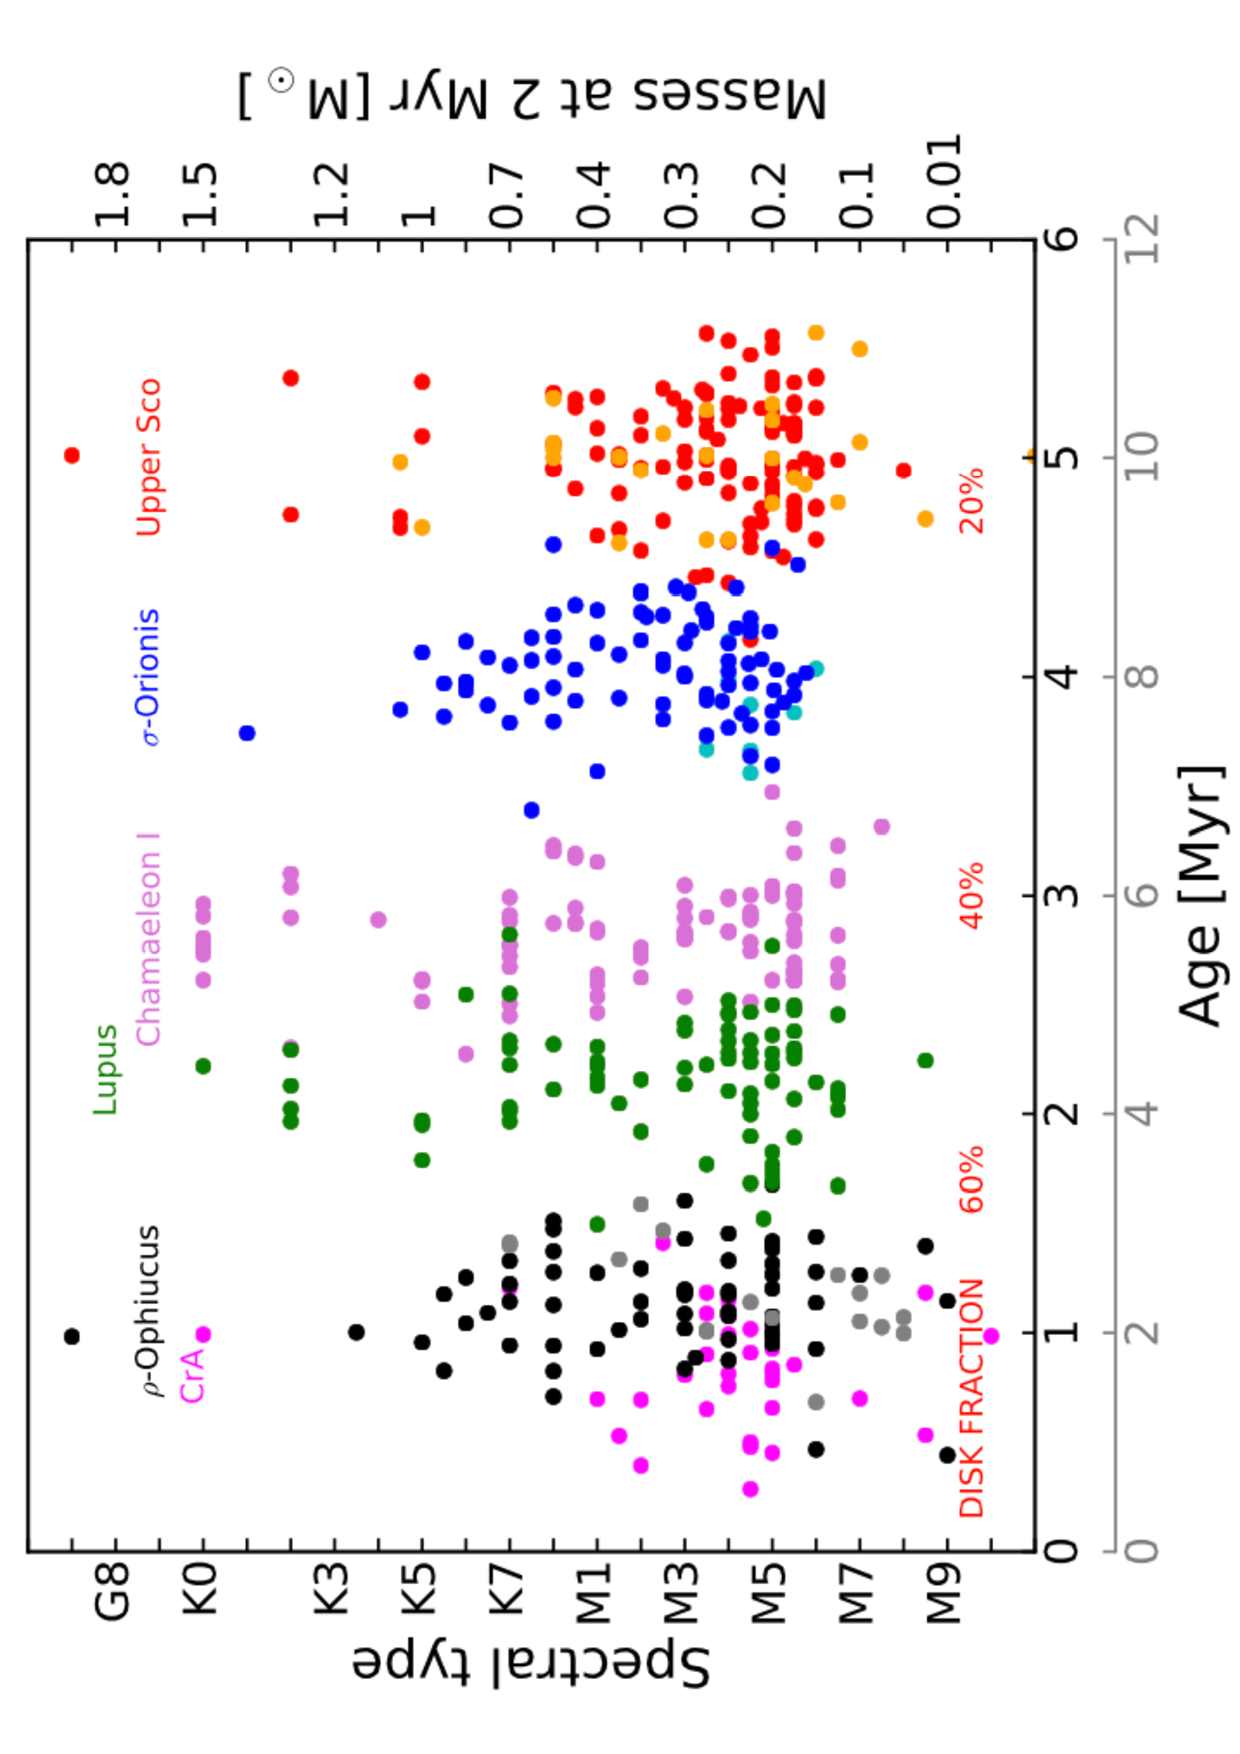
\includegraphics[scale=0.4,angle=-90]{f_samples_alma.pdf}}
\caption{Samples for which ALMA observations of disks will be available for this project. The spectral types are actual measurements; the ages are assigned randomly to each point using the mean age and age dispersion in each region.}
\label{f_almasamp}
\end{figure}

\vspace{1em}{\Tcol\bf ALMA Data for objective O4, O5 and O6}.

Objective O4 requires a combination of high angular resolution and high sensitivity data, to be able to resolve the gaps and holes and to detect at sufficient signal to noise ratio. There are several datasets either in the ALMA archive or scheduled to be observed that can be used. We will initially focus on three objects, in different evolutionary stages, for which detailed ALMA and VLA observations are available and for which we have acquired, or are in the process of acquiring, complementary high-contrast infrared observations: the young disk in HL~Tau, the full disk HD163296, and the TD around CQ~Tau.

All three objects already have, or we expect to receive in early 2017 from ALMA and the VLA, multi-wavelength continuum observations that allow us to trace the dust properties at different disk locations. Our own and archival datasets will also provide observations of the molecular gas in the three objects.
The initial modeling results that we aim to verify is that these three disks are in different stages of the planet formation process: HL~Tau contains rocky cores of planets that can effectively create gaps in the dust, but not in the gas surface density; HD163296 has sub-jupiter planets able to open gaps of varying depth in the dust and gas distributions; CQ~Tau contains large planets and is in an advanced phase of disk dissipation.

A summary of the available data on these three disks is shown in Figure~\ref{f_nir_alma}, including the complementary high-contrast imaging data that our team is acquiring to complement this project. In addition to these three disks, for which our team has direct access to available or planned multi-wavelength ALMA and VLA observations, we are in the process of securing additional high-contrast NIR imaging and high-resolution ALMA observations for an extended sample of five additional disks (2 TDs and 3 full disks), for which ALMA data exist or observations are planned.

\begin{figure}
\centerline{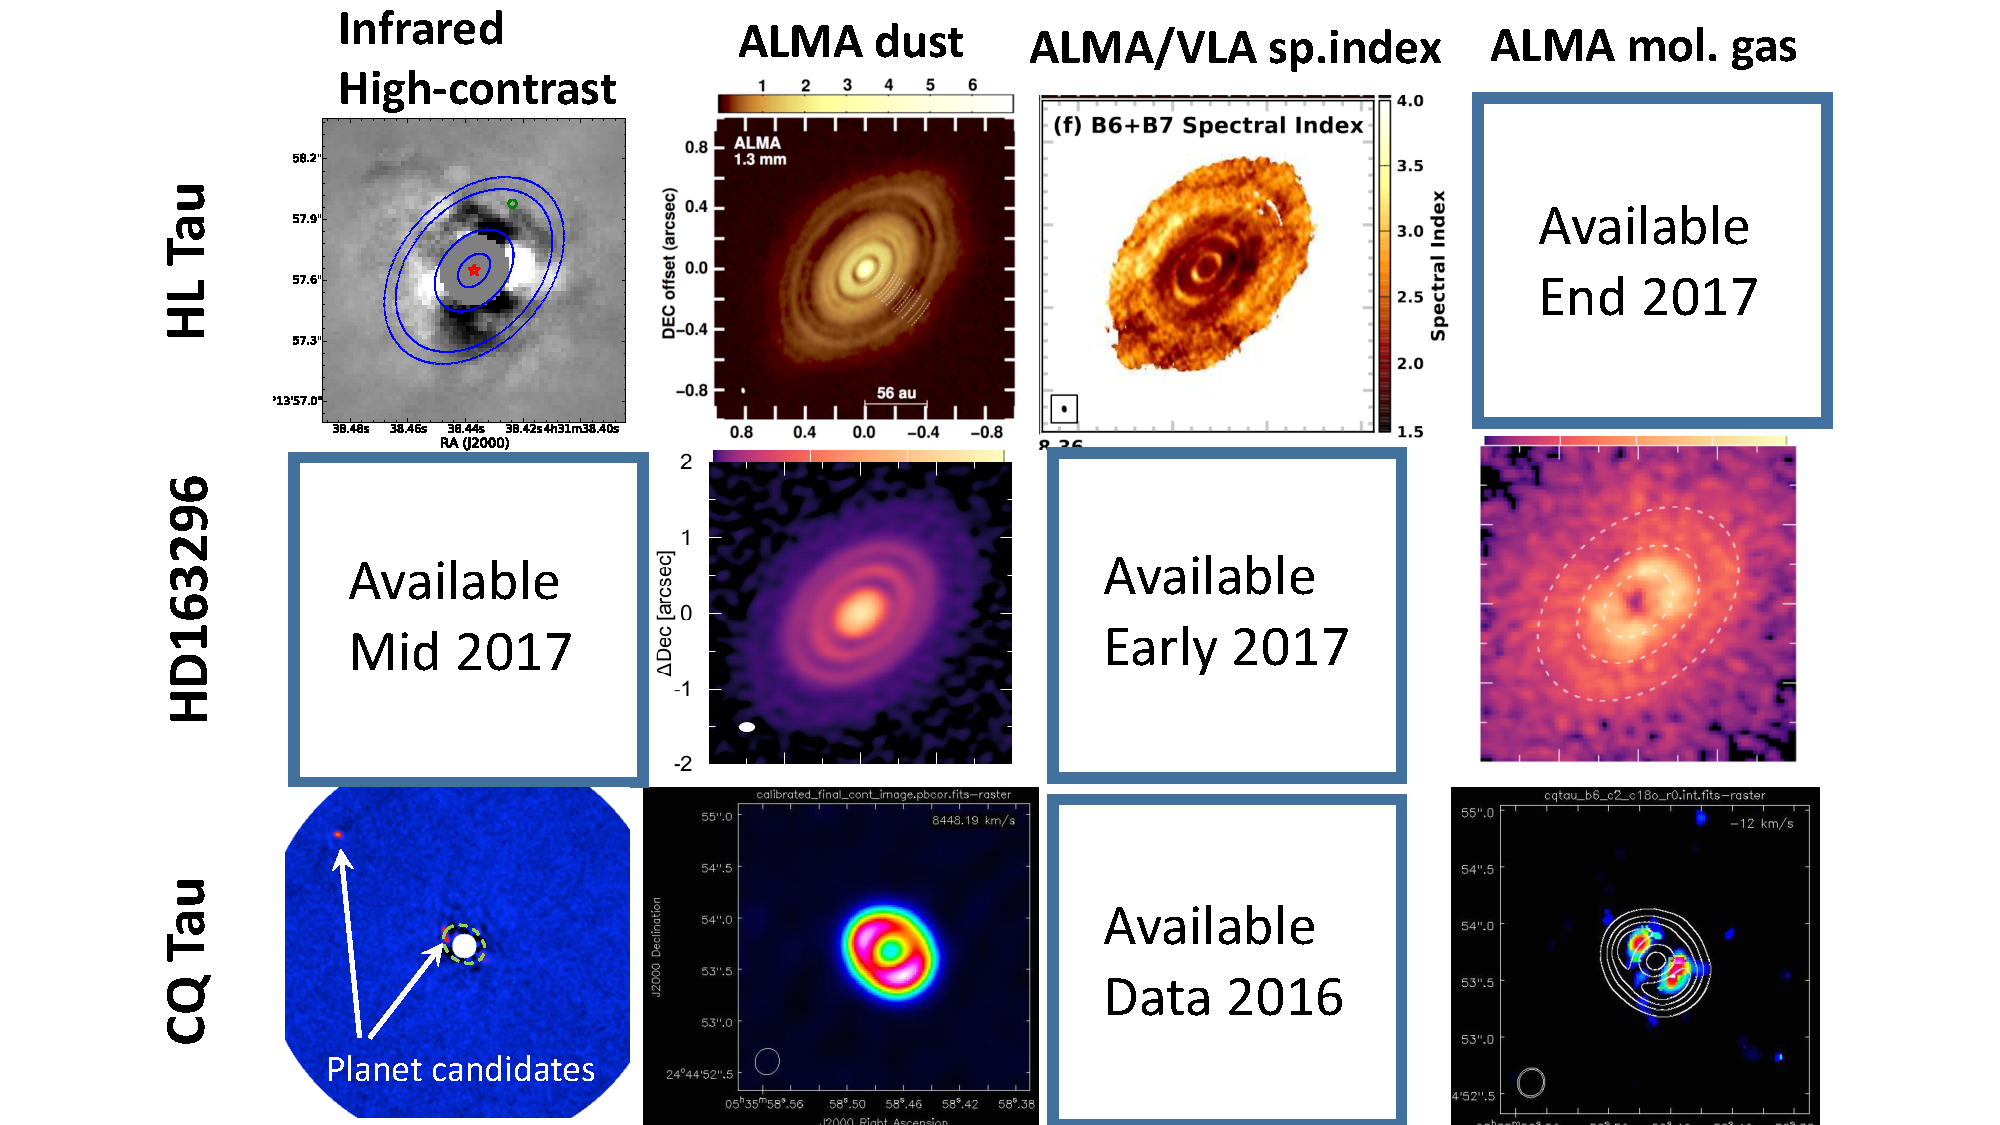
\includegraphics[scale=0.4,angle=0]{f_highres_data.pdf}}
\caption{\caphighlight{From Top to Bottom:} 
  %available data for HL~Tau,
  %HD163296 and CQTau. In \caphighlight{each column} we show: the
  %complementary high-contrast infrared data to search for planetary mass
  %companions, the ALMA continuum image, the ALMA spectral index image, the
  %molecular line integrated image. On the high contrast images we show the
  %position of the gaps in HL~Tau (Testi et al.~2015), and the position of
  %the outer edge of the disk cavity in CQ~Tau (Testi et al., in
  %preparation); HD163296 will be observed at the Keck telescope with the
  %high-contrast imager in Jun~2017. The ALMA continuum images are at 1.3 or
  %0.89~mm (ALMA Partnership et al. 2015; Isella et al. 2016; Perez et al. in
  %preparation). New high sensitivity data from the VLA and ALMA will be used
  %to construct the spectral index maps for HD163296 and CQ~Tau (data being
  %acquired); several ALMA programs aiming at observing the gas distribution
  %in HL~Tau, HD163296, and CQ~Tau are in progress.
available data for HL~Tau, HD163296 and CQTau. In \caphighlight{each column} we show: the complementary high-contrast infrared data to search for planetary mass companions, the ALMA continuum image, the ALMA spectral index image, the molecular line integrated image. On the high contrast images we show the position of the gaps in HL~Tau (Testi et al.~2015), and the position of the outer edge of the 
disk cavity in CQ~Tau (Testi et al., in preparation); HD163296 will be observed at the Keck telescope with the high-contrast imager in Jun~2017. The ALMA continuum images are at 1.3 or 0.89~mm (ALMA Partnership et al. 2015; Isella et al. 2016; Perez et al. in preparation). New high sensitivity data from the VLA and ALMA will be used to construct the spectral index maps for HD163296 and CQ~Tau (data being acquired); several ALMA programs aiming at observing the gas distribution in HL~Tau, HD163296, and CQ~Tau are in progress.}
\label{f_nir_alma}
\end{figure}


\subsection{Tools for data analysis}
% for each applicant
\label{s_tools}

In the last few years, our group has been developing and testing new tools to analyse planet forming disk observations and derive the properties of the dust and gas components. The two main tools that we expect to use and improve as part of this project are described below. The tools have been developed as part of two PhD Thesis at LMU and Leiden University.

\vspace{1em}{\Tcol\bf Dust properties and surface density as a function of radius}\\
As part of the PhD thesis of M. Tazzari at LMU (completed at the end of 2016), under the supervision of the project PI and the Co-I Prof.Dr. B. Ercolano, we developed an effective analysis tool that can be used to derive the dust properties and surface density as a function of radius. The novel modeling toolkit, allows to efficiently model multi-wavelength continuum observations of disks at millimetre and radio wavelengths to self-consistently derive the disk physical parameters (including the dust surface density distribution) and the level of grain growth as a function of radius in the disk. This tool has been verified and successfully applied to observations of planet forming disks, allowing for a direct comparison with global dust evolution models in disks (Tazzari et al. 2016ab; Tazzari et al. 2017).  

The tool has three basic modules: a disk model, with parameters that describe the physical structure of the disk and of the dust population; an likelyhood calculator, which computes proper interferometric model visibilities and compares them with the data; and a highly efficient Markov Chain Monte Carlo sampler.
We already tested the code modular approach by using different disk models (e.g. Tazzari et al. 2016a; Guidi et al. 2016), and we have made a considerable effort (in collaboration with the Excellence Cluster `Universe' C2PAP in Munich and with the support of NVIDIA) to structure the likelyhood calculation and the MCMC sampler to fully use a multi-CPU/multi-GPU architecture (developed on our data analysis server at ESO and fully tested on the HYDRA cluster as part of the collaboration with Prof. Dr. P. Caselli group at MPE). This effort allows to run effective multi-wavelength analysis on large samples (typical full analysis time is currently 24hrs/disk with observations at four wavelengths), and opens the possibility of expanding the analysis to the fit of multiple velocity channels for simple line emission models. 

\vspace{1em}{\Tcol\bf Disk gas masses from ALMA observations}\\
As part of her PhD thesis at the University of Leiden (to be completed in 2017) and under the supervision of project Co-I Prof. Dr. E. van Dishoeck, A. Miotello is developing an accurate method to measure the amount of molecular gas protoplanetary disks from CO and isotopologues millimetre observations. To overcome some of the difficulties in in deriving reliable gas surface densities from observations of line intensities, the method relies on a detailed chemical-physical computation of the disk dust and gas structure, including selective effects on the CO isotopologues. Miotello et al.~(2016) have used this method to derive measurements of the molecular gas content in disks using a combination of line luminosities in different CO isotopologues, improving on the method of Williams \& Best~(2014).

The application of this method to the Lupus ALMA disks survey (Miotello et al. 2017, see also Fig.~\ref{f_LADS}) has shown a significant inconsistency between the disk masses measured using dust or CO as tracers. This inconsistency could be related to a real deficit of the gas content in the Lupus disks, or to unexpected chemical depletion of CO and isotopologues. In collaboration with the Lupus team, and as part of the last part of A. Miotello PhD, we are exploring which of these two possibilities is correct using multi-transition CO and isotopologues data coming from approved ALMA programmes. This new analysis will be used to improve the method in the course of 2017. In collaboration with the group of J. Williams in Hawaii, we also plan to expand the method to derive gas surface densities for spatially resolved observations of gaseous disks.

\subsection{Work programme including proposed research methods}
% for each applicant
\label{s_work}


\todo{Kees to Leonardo: Please add into the text something about the role of
  the co-Is and other RU collaborators. Thomas Henning and Ewine van
  Dishoeck have of course loads of exciting data from SPHERE (Thomas) and
  ALMA (Ewine). It would be perhaps nice to see if you can find a way to
  link their expertise somehow (at least a bit) into this project. And what
  about adding Til, since his expertise may be useful to interpret the
  observations? Link to project C1 perhaps? For the gas phase tracers maybe
  you can refer to the expertise of Paola's group and Ewine's group on the
  chemistry of the gas in the disk, and link to project B2?}



The two PhD students hired for this project will each be responsible for one of the two main sub-project:
evolution of the demographics of disk properties and evolution of the detailed physical properties of disks with embedded planets. The workplan for the two sub-projects is detailed below.

\subsubsection{Evolution of the demographics of disk properties}

{\Tcol\bf Months 1-12}\\

We will start with the detailed analysis of the continuum properties of the Lupus disks from the combination of the ALMA surveys at 0.89, 1.3 and 3~mm. Dust emissivity, surface density and temperature
distributions are key uncertainties when deriving disk dust masses from sub-mm observations. The combination of the multi-wavelength observations of the Lupus disks will allow to greatly reduce the 
uncertainties. Using the modeling tool described in Sect.~\ref{s_tools}) we have already investigated the
possibility of refining the dust mass estimates by applying a correction that depends not only on the stellar luminosity (see the attempts by Andrews et al.~2013 and van der Plas et al.~2016), but also on other parameters like the radial extent of the millimetre wave emission (Tazzari et al.~2017). These initial results need to be validated using the multi-wavelength sample, in order to check for potential systematic effects introduced by the varying dust properties (see e.g. Banzatti et al. 2011; Tazzari et al. 2016a). All the data for this analysis is available, as the data has been delivered at the end of 2016. We also expect that at the beginning of the project all Lupus datasets will be already calibrated and ready for analysis.

The modeling procedure is already fully developed and tested on the single wavelength Lupus data, the key result that we will obtain for each modeled disk, once we add the multi-wavelength observations, will be: the total disk mass, the average dust properties (and possibly an indication of the dust properties as a function of radius), and the radial extent of the disk containing the bulk of the dust mass. The collaboration with M. Tazzari, will be crucial in this phase of the project and the student may spend 
some time (4-6 weeks) visiting the Institute of Astronomy in Cambridge (UK), where Tazzari is not a postdoc. From our initial results on the Lupus 0.89~mm survey, we estimate that  we will be able to carry out this analysis to almost half of the Lupus sample ($\sim 35$ disks). This sample contains 7-10 TDs (seven previously known, plus three that we have preliminarily reclassified as TDs), so we will also be in the position of addressing a first systematic assessment of the comparison of dust properties of TDs versus full disks.

During this period the student will also learn how to prepare the data from the other surveys available for this analysis. 
We will collect and re-process the ALMA data in a uniform way and, for all regions, we will use the optical/infrared spectroscopic data and methodology of Pascucci et al.~(2016) to recompute the stellar parameters, as this is a more robust 
technique than the one used in the initial studies of Barenfeld et al.~(2016) and Ansdell et al.~(2016).

Single wavelength data for the dust continuum emission and stellar parameters will be available at the end of this period for the following star forming regions (on top of Lupus): Corona Australis, Chamaeleon~I, $\sigma$-Orionis, Upper Scorpius. The line data will also be calibrated, but not analysed yet, at this stage. Observing proposals will be submitted to ALMA to expand the multi-wavelength samples, and additional data may become available, but it will not be critical for the success of the project.

\smallskip
{\bf Products:} 
\begin{itemize}
\item One publication on the dust properties and continuum masses in the Lupus cloud, including a comparison between full disks and TDs.
%\item One publication on the detailed analysis of the dust properties in HD163296 and/or CQ Tauri
\item ALMA proposal to extend the studies of the multi-wavelength dust properties to other regions beyond Lupus and Upper Sco
\item Datasets and methods ready for the comparative analysis of different star forming regions
\end{itemize}

{\Tcol\bf Months 13-24}\\

We will develop the statistical tools to compare the dust measurements in the different regions.
Different regions have different properties in terms of the stellar populations, fractions of stars with disks and completeness of the surveys. These limitations have not been taken fully into account in previous 
comparisons between the properties of disks in different star forming regions (e.g.\ Ansdell et al.~2016; Pascucci et al.~2016). To take into account the sampling and completeness biases, we will compare observational data to Monte Carlo simulations, building on and extending the methodology developed by Andrews et al.~(2013).  

The comparative study of the properties of the continuum emission of all star forming regions planned in this study will be completed in this phase. This will include the disks in $\rho$-Oph if the ALMA data will be available in time. 

The database will be extended to include the molecular line maps of the disks.
 
\smallskip
{\bf Products:} 
\begin{itemize}
\item One publication on the comparative properties of dusty disks in star forming regions as a function of age, including a comparison between full disks and TDs (achieving objectives {\bf O1} and {\bf O2}).
%\item One publication on the detailed analysis of the comparative properties at high angular resoltion of the disks HL~Tau, HD163296 and CQ Tauri
\item Statistical methods ready to be applied to the analysis of the gas properties
\end{itemize}

{\Tcol\bf Months 25-36}\\

The demographical analysis of the gas properties will be carried out during the third year. This analysis will be carried out as part of the collaboration with A. Miotello and J. Williams, using the methods that are currently being refined and are described in Sect.~\ref{s_tools}. For this analysis we will use the simplified fitting functions, rather than performing a full chemical modeling of each disk, which would be a prohibitively time consuming activity if applied to all the disks in our surveys. The fitting functions provided by Miotello et al.~(2016) will be improved following the ongoing studies (as described in Sect.~\ref{s_tools}), in addition, as part of our collaborations, we are planning to extend the model grids for a range of the stellar photospheric parameters. These new grids will be applied to derive more accurate measurements of the gas content to be compared with the solids content in disks as a function of the evolutionary status. As part of the outcome of this analysis we will also compare the results of the 
analysis of the gas in disks with the measurements of the $M_{acc}$ as derived from our optical spectroscopy database.

\smallskip
{\bf Products:} 
\begin{itemize}
\item One publication on the comparative properties of the gas content in disks in star forming regions as a function of age, including a comparison between full disks and TDs (achieving objective {\bf O3}).
%\item One publication on the detailed analysis of the comparative properties at high angular resoltion of the disks HL~Tau, HD163296 and CQ Tauri
\item Investigation of the possible evolution of the overall gas-to-dust ratio in disks as a function of age, evolutionary stage and stellar parameters; with particular emphasis on determining possible population differences between full disks and TDs
\end{itemize}

\subsubsection{Evolution of the detailed physical properties of disks with embedded planets}

{\Tcol\bf Months 1-12}\\
In this first phase we will collect and reprocess the ALMA and VLA high angular resolution observations of CQ~Tauri amd HD163296 (the HL~Tau continuum data are already available). The expert postdoctoral Fellow at ESO and collaborator on this project (Baobab Liu) will support this data calibration effort.

The most significant part of the time will be used to modify the model part of the multi-wavelength analysis tool to incorporate a fast (parametric) computation of the line emission. We have already developed a parametric model to describe line emission for our recent work on HD163296 (Isella et al.~2016), and we plan to incorporate an optimized version of this model in the analysis tool. 
We will develop this as part of the multi-CPU/multi-GPU version of the analysis code.  The main modifications that we will implement in the model are a parametric description of the position of gaps and holes in the disk and the associated gas and dust depletion factors; a version that allows for an analysis of gaps and rings in the dust emission is already working (e.g. Guidi et al.~2016), but we need to add the modifications required for the analysis of the gas.

\smallskip
{\bf Products:} 
\begin{itemize}
\item New version of the analysis code with incorporated the model required to perform a parametric analysis of the dust and gas emission in disks with gaps and holes
%\item One publication on the detailed analysis of the comparative properties at high angular resoltion of the disks HL~Tau, HD163296 and CQ Tauri
\item One publication describing the application of the analysis tool to one disk observed at high angular resolution with ALMA
\end{itemize}

{\Tcol\bf Months 13-24}\\
%The analysis of the disks observed at high angular resolution and high sensitivity multi-wavelength ALMA observations and complementary high-contrast near infrared imaging will be completed, applying the modeling tool modified in the first phase of the project. We will also incorporate the results of the analysis
%methods for the gas to derive a reliable measurement of the gas surface density in these disks. 
%The data will be compared with models developed as 
%part of other projects in the RU to understand if the different dust 
%and gas properties and the potential detection of planetary mass companions are consistent with an evolutionary scenario. The data will constrain the model predictions for the development of gaps (in dust and gas) in the two full disks, and the hole and dust/gas properties in the TD.

Depending on the progress of the high-contrast imaging survey and the quality of the data for resolved disks in the ALMA archive and our own programmes, we may expand the study to additional disks observed at high angular resolution. 

\vspace{1em}{\Tcol\bf Months 25-36}\\
The analysis of the disks observed at high angular resolution and high sensitivity multi-wavelength ALMA observations and complementary high-contrast near infrared imaging will be completed, applying the modeling tool modified in the first phase of the project. We will also incorporate the results of the analysis
methods for the gas to derive a reliable measurement of the gas surface density in these disks. 
The data will be compared with models developed as 
part of other projects in the RU to understand if the different dust 
and gas properties and the potential detection of planetary mass companions are consistent with an evolutionary scenario. The data will constrain the model predictions for the development of gaps (in dust and gas) in the two full disks, and the hole and dust/gas properties in the TD.

\subsection{Data handling}

ESO is acquiring a dedicated computing cluster for the processing of science data from ALMA (and other observatories/instruments). The computing cluster architecture is copied from the ALMA Regional Centre Cluster architecture, this ensures that all ALMA data processing applications can be used and will work at peak efficiency. We expect to have direct access to this system once will be installed and open to the ESO astronomers (expected by February 2017). 

Our group at ESO has direct access to a high-end server that we used for the analysis of the Lupus disks presented in Tazzari et al.~(2017). This server has an hybrid multi-CPU (2 CPUs with 14 compute cores, each capable of double threading), multi-GPU (2 NVIDIA Tesla-K40) architecture that we used to develop and test the advanced data analysis software developed in Tazzari~(2016b). 

We have access to, and we will continue to use for this project, the computing facilities in the Garching campus offered by the Excellence Cluster (the C2PAP cluster) and the Max Planck Institutes (the Hydra cluster). We have already been using these facilities to successfully and effectively model the dust properties and distribution in protoplanetary disks (Guidi et al. 2016; Tazzari et al.~2016a; Tazzari et al. 2017).

Given the large amount of data analysis for this project, we will need to upgrade the fast-io storage of the server in our group, which is required for effective ALMA data processing in CASA. In addition we require a high-end desktop computer with a large data storage external drive for post processing and analysis of the data. To share data and analysis results with the rest of the team, we plan to use one of the commercially available cloud storage services (e.g.\ Dropbox, GoogleDrive, OneDrive, etc). 

As part of this project, we will make available the re-processed ALMA data via a dedicated website. The data will be released in progressive instalments together with the publication of the research papers.

% \subsection{Other information}
% % Please use this section for any additional information you feel is
% % relevant which has not been provided elsewhere.
% 
% [Text]
% 
% \subsection{Information on scientific and financial involvement of international cooperation partners}
% 
% [Text]

\section{Bibliography}

%\begingroup
%\renewcommand{\section}[2]{}%
%%\bibliographystyle{icarus}
%\bibliographystyle{aa}
%\bibliography{A1}
%\endgroup


ALMA Partnership, Brogan C., et al. 2015, ApJ 808, L3\\
Andrews S.W., Wilner D.J., Espaillat C., Hughes A.M., Dullemond C.P., et al. 2011, ApJ 732, 42\\
Isella A., Guidi G., Testi L., et al. 2016, PhysRevLett in press\\
Lommen D., Wright C.M., Maddison S.T., et al. 2007, A\&A 462, 211\\
P\'{e}rez L., et al. 2016, Science 353, 1519\\
Pinilla P., Benisty M., Birnstiel T., Ricci L., Isella A., Natta A., Dullemond C.P., Quiroga-Nunez L.H., Henning T., Testi L. 2014, A\&A 564, 51\\
Ricci L., Testi L., Natta A., Brooks K.J. 2010a, A\&A 521, 66\\
Ricci L., Testi L., Natta A., et al. 2010b, A\&A 512, 15\\
Sallum S., Follette K.B., Eisner J.A., Close L.M., Hinz P., et al. 2015, Nature 527, 342\\
Ubach C., Maddison S.T., Wright C.M., et al. 2012, MNRAS 425, 3137\\
van der Marel N., van Dishoeck E.F., Bruderer S., P\'{e}rez L., Isella A. 2015, A\&A 579, 106\\
van der Marel N., Verhaar B.W., van Terwisga S., Mer\'{i}n B., et al. 2016a, A\&A 592, 126\\

\section{Requested modules/funds}
\renewcommand{\leftmark}{\sc  Requested modules/funds}
% Explain each item for each applicant (stating last name, first name).

\subsection{Basic Module}

\subsubsection{Funding for Staff}
% Please note that funds for your own temporary position (“Eigene Stelleâ€)
% are not to be included here; this belongs to the separate “Module Temporary Positionâ€.

\todo{[Text]}

\todo{Barbara: do we need to put the cost of the student here? Answer from
  Kees: yes. Salary group E13, either 75\% or 50\%. This is, by the way,
  something we have to decide for the entire Forschergruppe: do we do 50\%
  or 75\% contracts for PhD students?}

\subsubsection{Direct Project Costs}

\todo{[Text]}

\paragraph{Equipment up to EUR 10,000, Software and Consumables}

\begin{itemize}
\item {\bf desktop:} high-end desktop for ALMA data analysis (4k\EUR{}) 
\item {\bf storage:} upgrade of the ESO data reduction server fast-io storage (3k\EUR{})
\item {\bf storage:} external slow (e.g. USB disk) large storage (30Tb class) for project data (1.5k\EUR{})
\item {\bf storage:} cloud storage service for collaboration data sharing (1.5k\EUR{})
\end{itemize}

Total equipment cost: 10k\EUR{}  

\paragraph{Travel Expenses}

During the project we expect an average of 1 intercontinental and 2 european
trips per year to work with the collaborators, plus 1 intercontinental and 2
european trips to present results at conferences and meetings. The expected
cost is 3k\EUR{} for each intercontinental trip (note that one of the
collaborators is in Hawaii and one in Santiago de Chile, implying relatively
expensive airfares) and 1k\EUR{} for each european trip. So for a total of
4 intercontinental and 8 european trips, we expect a total of 20k\EUR{}.  \smallskip

Total travel expenses: 20k\EUR{}


\paragraph{Visiting Researchers (excluding Mercator Fellows)}

Given the distributed nature of the collaboration, including collaborators in USA and Chile, we expect to host 2 1-week visits per year. Typically, we expect each visit to cost 0.5-1k\EUR{}, depending on the trip details and assuming that these visits will be connected to other trips to Europe for the overseas visitors (which would then require just an intra-european trip extension). We thus estimate a total expense of 5k\EUR{}.
\smallskip

Total travel expenses: 5k\EUR{}

\paragraph{Other Costs}

Given the distributed nature of the collaboration, we expect to organize one team meeting in 
Munich for this sub-project. We thus require funding to cover the general expenses of the 
organization of the meeting (2k\EUR{}).\smallskip
 

Total other expenses: 2k\EUR{}

\paragraph{Project-related publication expenses}

Given the distributed nature of the collaboration, it may be necessary to contribute to publication expenses for overseas journals (e.g.\ the Astrophysical Journal). \smallskip

Total publication expenses: 1k\EUR{}

\subsubsection{Instrumentation}

\todo{[Text]}

\paragraph{Equipment exceeding EUR 10,000} 

\todo{[Text]}

\paragraph{Major Instrumentation exceeding EUR 100,000} 

\todo{[Text]}

% \subsection{Module Temporary Position}
% 
% [Text]
% 
% \subsection{Module Replacement Funding}
% 
% [Text]
% 
% \subsection{Module Mercator Fellows}
% 
% [Text]
% 
% \subsection{Module Public Relations Funding}
% 
% [Text]

\section{Project requirements}
\renewcommand{\leftmark}{\sc Project requirements}

\subsection{Employment status information}
% For each applicant, state the last name, first name, and employment
% status (including duration of contract and funding body, if on a
% fixed-term contract).

\todo{[Text]}

%\subsection{First-time proposal data}
%% Only if applicable: Last name, first name of first-time applicant.
%
%[Text]

\subsection{Composition of the project group}
% List only those individuals who will work on the project but will not
% be paid out of the project funds. State each person’s name, academic
% title, employment status, and type of funding.

\todo{[Text]}

\subsection{Cooperation with other researchers}

\subsubsection{Planned cooperation on this project}

\paragraph{Collaborating researchers for this project within the
  Research Unit}
%Each proposal must be accompanied by a description of how the project
%is integral to the Research Unit, %both in terms of subject matter
%and organisation. This includes a description of the cooperation with
%%others participating within the Research Unit. 

\todo{Please summarize here how this project is linked to the other RU
  projects.}

\paragraph{Collaborating researchers for this project outside of
  the Research Unit}

\todo{Please summarize here how this project is linked to international
  teams.}


\subsubsection{Researchers with whom you have collaborated scientifically within the past three years}
% This information is important for DFG to exclude possible conflicts of interest.
% Please mention not only the names of the cooperation partners but also their institution and city.
% Scientists already mentioned in the previous two subsubsections do not have to be mentioned
% again.

\todo{Please just provide a list of names. Kees to Leonardo: in your case
  this list is too long. So please only put the names of people you
  collaborate with closely.}

\subsection{Scientific equipment}
% List larger instruments that will be available to you for the
% project. These may include large computer facilities if computing
% capacity will be needed. 

\todo{[Text]}

\subsection{Project-relevant interests in commercial enterprises}
% Information on connections between the project and the production
% branch of the enterprise.

\todo{[Text]}


\subsection{Additional information}
% If applicable, please list proposals requesting major
% instrumentation and/or those previously submitted to a third party
% here.

\todo{[Text]}


\end{document}
